\chapter{???}
\todo[author=Nozik, inline]{Название главы?}

Электрический ток представляет собой направленный перенос зарядов. Микрочастицы, осуществляющие этот перенос, называют {\textsf{носителями тока}}. В простейшем случае (ток в вакуумном диоде, ионный пучок в масс-спектрометре, и т.~д.) носителями тока являются заряженные частицы, движущиеся в свободном от вещества пространстве. Чаще всего такими частицами являются электроны~--- элементарные частицы с известными значениями заряда и массы.

Понятие \textsf{носители тока в веществе} уже не является таким простым и наглядным. Хотя в металлах и полупроводниках перенос заряда происходит вследствие перемещения всё тех же электронов, их движение уже не является движением свободных частиц, как в вакууме. Теперь электроны движутся в сильном периодическом поле, образованном ионами кристаллической решётки, и взаимодействуют между собой, причём это движение и это взаимодействие подчиняются законам квантовой механики. По этим законам получается, что такое движение можно по-прежнему интерпретировать как движение свободных заряженных частиц, но масса этих частиц, называемая эффективной массой, не совпадает с массой свободного электрона. Более того, в полупроводниках и в некоторых металлах простые законы движения получаются только в том случае, если вместо электронов ввести фиктивные частицы~--- так называемые \textsf{дырки}. Дырки подобны элементарным частицам позитронам,то есть в электрических и магнитных полях они движутся как положительно заряженные частицы с зарядом, численно равным заряду электрона, но правда с некоторой эффективной массой (не равной массе электрона).

Таким образом, в физике металлов и полупроводников в качестве носителей тока рассматривают квазичастицы, не существующие в природе отдельно от рассматриваемого вещества. Заряд этих носителей численно точно равен заряду электрона и может быть как отрицательным, так и положительным. В первом случае они по-прежнему называются электронами (хотя их масса, как уже говорилось выше, не равна массе электрона), во втором~--- дырками. В полупроводниках присутствуют оба типа этих носителей, в большинстве металлов имеются только отрицательные носители, причём по классической теории электропроводности в качестве таковых рассматривают обычные свободные электроны.

{\bf \Large Определение элементарного заряда}

Первые точные измерения элементарного заряда были выполнены Робертом Милликеном в классических опытах в 1908--1916 годов. Идея этих опытов достаточно проста. Если элементарный заряд действительно существует, то величина заряда $q$ любого тела может принимать только дискретную последовательность значений:
$$q = 0,\,\pm e,\,\pm2e,\,\pm3e,\,\pm4e, \ldots,\, \pm ne,\, \ldots,
$$
где $e$~--- элементарный заряд (\emph{абсолютная} величина заряда электрона).

В опыте Милликена измеряется электрический заряд капелек масла микроскопических размеров, несущих всего несколько
элементарных зарядов. Сравнивая между собой заряды капель, можно убедиться в том, что все они кратны одному и тому же числу, которое и равно, очевидно, заряду электрона.

Измерение заряда капель производится путём исследования их движения в электрическом поле. В расположенный горизонтально плоский конденсатор через отверстие в верхней пластине впрыскиваются мелкие капельки масла, получаемые с помощью специального распылителя. На пластины конденсатора подаётся постоянное напряжение (несколько киловольт). В ходе опыта это напряжение можно изменять. При распылении капельки масла вследствие трения о воздух приобретают случайный по величине и знаку электрический заряд. Попадая в конденсатор, капельки масла движутся в воздухе, опускаясь под действием силы тяжести или поднимаясь под действием электрического поля. Время $t_0$ опускания капли и время её обратного подъёма $t$ легко измерить с необходимой точностью. Оказывается, что именно к измерению этих двух интервалов времени и сводится измерение заряда капли.

Разумеется, дискретность заряда разных капель и, следовательно, величина элементарного заряда, то есть заряд электрона, могут быть обнаружены только в том случае, если абсолютная ошибка в измерении заряда капли будет существенно меньше самого элементарного заряда. В опытах Милликена необходимая точность вполне может быть обеспечена в условиях лабораторного практикума.

{\bf \Large Движение заряженных частиц в электрических и~магнитных полях}

Рассмотрим несколько примеров движения электронов в вакууме под действием электрического и магнитного полей. Такие
условия движения реализуются, например, в электронных вакуумных приборах, таких, как электронно-лучевая трубка или
вакуумный диод.

Эти относительно несложные и наглядные примеры позволят нам понять, как можно измерить такую важную характеристику
заряженной частицы, как отношение её заряда к её массе $e/m$ (удельный заряд частицы).

{\bf \large   Движение электрона в однородном магнитном поле}

\label{2.1}%

Как известно, на заряд $q$, движущийся со скоростью $\vec{v}$ в магнитном поле $\vec{B}$, действует сила Лоренца:
$$
\vec{F}=q{\vec{v}}\times{\vec{B}}.
$$
Пусть электрон движется с некоторой скоростью $\vec{v}$ в однородном магнитном поле, индукция которого $\vec{B}$
перпендикулярна направлению скорости. На движущийся электрон действует сила %Лоренца, равная, как известно,
\begin{equation}
%12g
\vec{F}=-e{\vec{v}}\times{\vec{B}},
\end{equation}
где $e$~--- абсолютная величина заряда электрона. Эта сила перпендикулярна скорости движения и не изменяет поэтому её абсолютной величины. Траектория движения электрона в этом случае является окружностью. Такое движение частицы называется циклотронным вращением. Вычислим радиус $R$ этой окружности, называемый \textsf{ларморовским радиусом} электрона, и угловую скорость циклотронного вращения $\omega_c$~--- так называемую \textsf{циклотронную частоту}.

Сила $F$ является центростремительной силой, поэтому
$$
m\frac{v^2}{R}=evB,
$$
откуда
\begin{equation}
%13g
R =\frac{v}{\omega_c},
\end{equation}
где
$$
\omega_c=\frac{eB}{m}
$$
---~циклотронная частота электрона. Важно заметить, что циклотронная частота не зависит от энергии частицы, так что в однородном магнитном поле все электроны, находящиеся в рассматриваемом объёме, вращаются с одинаковой частотой.

Скорость движения электрона можно найти, зная разность потенциалов $V$, пройденную электроном:
$$
\frac{mv^2}{2}=eV,
$$
откуда
\begin{equation}
%14g
v=\sqrt{\frac{2eV}{m}} = 6\cdot10^5\sqrt{V}~\frac{m}{c}.
\end{equation}

Пусть теперь электрон движется в магнитном поле под некоторым углом $\alpha$ к вектору индукции. Скорость электрона
$\vec{v}$ можно разложить на две составляющие, одна из которых перпендикулярна, а другая параллельна магнитному полю:
$$
v_{\bot}=v\sin\alpha,\qquad v_{\parallel}=v\cos\alpha.
$$
Параллельная составляющая скорости не вызывает появление силы Лоренца, поэтому проекция траектории электрона на
плоскость, перпендикулярную $\vec{B}$, по-прежнему представляет собой окружность с ларморовским радиусом, определяемым поперечной составляющей скорости:
\begin{equation}
%15g
R =\frac{mv_{\bot}}{eB}.
\end{equation}
В направлении поля $\vec{B}$ на электрон не действуют никакие силы, следовательно, в этом направлении электрон движется равномерно со скоростью $v_{\parallel}$. Траектория электрона представляет собой винтовую линию. Найдём расстояние $L$, которое проходит электрон в направлении вдоль поля за один оборот (шаг винтовой линии). Как нетрудно видеть, время одного оборота $T_c$, называемое циклотронным периодом, равно: $T_c=2\pi R/v_{\bot}$. Заменяя $R/v_{\bot}$ c помощью (\r{15g}), найдём
\begin{equation}
%16g
T_c =\frac{2\pi m}{eB}.
\end{equation}

За это время электрон проходит вдоль магнитного поля расстояние
\begin{equation}
%17g
L = v_{\parallel}T_c =\frac{2\pi v\cos\alpha}{(e/m)B}.
\end{equation}

Нас будет интересовать главным образом случай, когда углы невелики, т.е. $\cos\alpha \approx 1$:
\begin{equation}
%18g
L \approx \frac{2\pi v}{(e/m)B}.
\end{equation}

Таким образом, расстояние $L$ не зависит от угла $\alpha$ (для малых углов), так что все электроны, вышедшие из одной точки, после одного оборота вновь соберутся в одной точке (сфокусируются). Как следует из (\r{18g}), индукция поля $B$, при которой точка фокусировки отстоит от точки вылета на расстоянии $L$, зависит от величины $e/m$~--- удельного заряда электрона. Обозначим через $B_f$ индукцию магнитного поля, при которой наступает фокусировка. Используя (\r{14g}) и (\r{18g}), выразим удельный заряд электрона $e/m$ через $B_f$:
\begin{equation}
%19g
\frac{e}{m}=\frac{8\pi^2 V}{L^2B_f^2}.
\end{equation}

Эта формула положена в основу экспериментального измерения удельного заряда электрона по \textsf{методу магнитной
фокусировки}.

{\bf Large Движение электрона в скрещенных электрическом и магнитном полях}

В так называемом {\textsf{методе магнетрона}} отношение $e/m$ измеряется на основе исследования движения электрона в скрещенных электрическом и магнитном полях, перпендикулярных друг другу. Название метода связано с тем, что такая
конфигурация электрического и магнитного полей реализуется в магнетронах~--- генераторах электромагнитных колебаний
сверхвысоких частот.

\begin{figure}
%\fcris{v3_3}{g3}
\caption{Движение заряда в скрещенных полях}
label{fig3.0.3}
\end{figure}

Для уяснения идеи метода магнетрона, рассмотрим вначале движение заряда в <<плоском магнетроне>>, который можно
представить себе в виде плоского конденсатора, помещённого в магнитное поле так, что $\vec{E}\bot\vec{B}$ (рис \ref{fig3.0.3}). Приэтом отрицательная пластина конденсатора играет роль катода, положительная соответственно анода. Если бы магнитного поля не было, то все электроны, вылетевшие без начальной скорости из катода такого плоского диода, попадали бы на анод. При наличии магнитного поля траектории электронов искривляются, вследствие чего при достаточно большом магнитном поле ни один электрон не достигнет анода. Для заданного напряжения между катодом и анодом существует некоторое критическое значение магнитной индукции $B_{KP}$, при котором траектории касаются поверхности анода. Если $B<B_{KP}$, то все электроны достигают анода и ток через магнетрон имеет то же значение, что и без магнитного поля. Если же $B>B_{KP}$, то электроны не достигают анода и ток через лампу равен нулю.

Рассчитаем это критическое значение индукции магнитного поля. Уравнения движения электрона в нашем случае имеет вид
\begin{equation}
%21g
m\frac{dv_x}{dt}=ev_y B,
\end{equation}
\begin{equation}
%22g
m\frac{dv_y}{dt}=eE-ev_x B
\end{equation}
при начальных условиях $x(0)=y(0)=0$, $v_x(0)=v_y(0)=0$.

Непосредственной подстановкой несложно убедиться в том, что решением системы дифференциальных уравнений с заданными
начальными условиями является уравнение циклоиды (в параметрической форме):
\begin{equation}
%23g
x = vt - R\sin\omega t,\qquad y = R(1-\cos\omega t),
\end{equation}

где $ v=\frac{E}{B}$, $R=\frac{v}{\omega}=\frac{Em}{eB^2}$.

Касание анода происходит при $2R=d$ ($d$~--- расстояние между анодом и катодом). Этому значению соответствует
критическое поле
\begin{equation}
%24g
B_{KP}=\frac{\sqrt{2V}}{d\sqrt{e/m}}.
\end{equation}
Из последней формулы находим удельный заряд:
\begin{equation}
%25g
\frac{e}{m}=\frac{2V}{d^2B_{KP}^2}.
\end{equation}

Эта формула позволяет вычислить $e/m$, если при заданном значении напряжения на аноде $V$ найти такое значение
магнитного поля, при превышении которого ток в магнетроне отсутствует.

{\bf \Large Электрический ток в вакуумном диоде}

Электрический ток в вакуумном диоде представляет собой упорядоченное движение электронов, испускаемых накалённым
катодом. Явление испускания электронов поверхностью твёрдого тела или жидкости называется {\textsf{электронной эмиссией}}.
Существует несколько видов электронной эмиссии. В частности, в случае испускания электронов поверхностями нагретых тел эмиссия называется {\textsf{термоэлектронной}}.

Одним из ключевых понятий, лежащих в основе объяснения явления электронной эмиссии, является понятие {\textsf{работы выхода}}. Под работой выхода понимают работу, которую необходимо совершить для удаления электрона из твёрдого вещества в вакуум в состояние с равной нулю кинетической энергией. В случае термоэлектронной эмиссии работа выхода совершается за счёт кинетической энергии электронов, которой они обладают внутри тела. У чистых металлов работа выхода составляет несколько электрон-вольт.

При повышении температуры металла увеличивается энергия теплового движения электронов, количество быстрых электронов и заметное их количество сможет преодолеть задерживающее электрическое поле и выйти из металла. Если приложить
электрическое поле, направленное к поверхности металла, то оно будет увлекать вышедшие электроны и через вакуум потечёт электрический ток. Этот ток называется {\textsf{термоэлектронным}}.

При холодном катоде ток через диод при подаче на анод положительного потенциала практически отсутствует. Если же нагреть катод, то в диоде возникает заметный ток. Ток прекращается при изменении полярности батареи. Это как раз и указывает на то, что носителями тока в диоде являются отрицательно заряженные частицы, а именно электроны.

Если бы все электроны, вылетающие из поверхности катода, попадали на анод, то сила термоэлектронного тока $I$ не
зависела бы от величины приложенного напряжения $V$. На самом деле это не так. С возрастанием напряжения ток растёт.
Однако возрастание идёт не пропорционально $V$, так что закон Ома для вакуумного диода не выполняется. При достижении определённого напряжения дальнейшее нарастание тока практически прекращается. Ток достигает предельного значения,называемого током насыщения. Величина тока насыщения определяется количеством электронов, которое способно выйти из поверхности катода в единицу времени и, следовательно, растёт с ростом температуры. Если электрическое поле настолько сильное, что способно отвести все эмитированные электроны, то дальнейшее увеличение напряжения уже не приводит к увеличению термоэлектронного тока. Этим объясняется явление насыщения тока.

Нелинейная зависимость тока от напряжения объясняется тем, что в пространстве между катодом и анодом образуется
отрицательный пространственный заряд, изменяющий распределение потенциала в диоде.

Допустим, что диод плоский, то есть его электроды представимы в виде двух параллельных плоскостей (расстояние между
электродами много меньше их площади). Направим ось $X$ перпендикулярно к поверхности катода в сторону анода, совместив начало координат с поверхностью катода. В этой модели задача стала одномерной~--- все величины являются функциями только координаты $x$. Потенциал электрического поля $\phi$ удовлетворяет уравнению Пуассона:
\begin{equation}
%01g
\frac{d^2\phi}{dx^2}=-\frac{\rho}{\epsilon_0},
\end{equation}

где $\rho(x)$~--- плотность электрического заряда. Плотность тока $j=\rho v$. Пренебрегая столкновениями электронов, их скорость можно определить из уравнения
$$
\frac{mv^2}{2}=e\phi.
$$

Начальными тепловыми скоростями, с которыми вылетают электроны с поверхности катода, здесь пренебрегается, а потенциал катода принимается равным нулю. Исключив из этих соотношений плотность электронов и скорость, приходим к уравнению
\begin{equation}
%02g
\frac{d^2\phi}{dx^2}=\sqrt{\frac{m}{2e\phi}}\, j.
\end{equation}

Для однозначного решения этого дифференциального уравнения второго порядка помимо условия $\phi(0)=0$ необходимо ещё одно граничное условие. Если сопоставить уравнения (\r{01g}) и (\r{02g}), то можно сделать вывод об обращении плотности заряда на катоде в бесконечность. Точка $x=0$ является особой точкой уравнения (\r{02g}), в которой оно теряет смысл.
Это связано с тем, что мы пренебрегли тепловыми скоростями на катоде, приняв их равными нулю. Оказывается, что в этой модели плотность тока через диод получается конечной, только если напряжённость поля у катода равна нулю. Это условие означает, что поле возникающего вблизи катода пространственного заряда полностью экранирует электрическое поле, создаваемое разностью потенциалов между анодом и катодом. Таким образом, получаем второе граничное условие в виде
$$
\left.\frac{d\phi}{dx}\right|_{x = 0}=0.
$$
Теперь задача о распределении потенциала становится однозначной и приводит к решению
$$
j=\frac{4\epsilon_0}{9x^2}\sqrt{\frac{2e}{m}}\phi^{3/2}.
$$
Так как $\phi(d)=V$, где $d$~--- расстояние между электродами, то для зависимости тока от напряжения получаем
$$
I=\frac{4\epsilon_0 S}{9d^2}\sqrt{\frac{2e}{m}}V^{3/2},
$$
где $S$~--- площадь катода. Мы получили зависимость тока через плоский диод от приложенного к нему напряжения, известную как <<закон трёх вторых>> для плоского диода. Оказывается, что не только для плоского вакуумного диода, а и для вакуумного диода с электродами любой другой геометрии ток подчиняется <<закону степени трёх вторых>>.

Полученная формула подсказывает очевидную процедуру измерения удельного заряда электрона. Для этого достаточно по
результатам эксперимента построить график зависимости тока от напряжения в степени трёх вторых, который должен
представлять собой прямую линию, проходящую через начало координат. Угол наклона этой прямой линии пропорционален (с известным коэффициентом) квадратному корню из $e/m$~--- искомой величины удельного заряда электрона.

{\large \bf Свободные носители заряда в металлах и~полупроводниках}

{\large  Зонная модель}

Проводимость большинства твёрдых тел связана с~движением электронов. Электроны входят в~состав атомов всех тел, однако одни тела не проводят электрический ток (диэлектрики), а другие являются хорошими его проводниками. Причина различия заключается в~особенностях энергетического состояния внешних электронов атомов в~этих веществах.

При объединении атомов в~твёрдое тело (кристалл) состояние внешние электроны теряют связь со <<своими>> атомами и теперь принадлежат всему кристаллу в~целом. Каждому уровню энергии электрона одиночного атома соответствует в~кристалле группа близких по энергии уровней (разрешённая зона), в~которой число уровней равно числу мест на соответствующем атомном уровне, умноженному на число атомов в~кристалле. Число уровней, объединившихся в~зону, при слиянии не меняется. Оно определяет максимальное число электронов, которое может <<поместиться>> в~зоне (в~силу принципа Паули).

Если одна из энергетических зон до конца заполнена электронами, а следующая зона совершенно пуста, то под действием слабого внешнего электрического поля электронам некуда перетекать, и вещество является \textsf{диэлектриком}. Верхняя из заполненных зон называется {\textsf{валентной зоной}}.

Положение меняется, если в кристалле имеется зона, частично заполненная электронами. В этом случае внешнее электрическое поле может изменить распределение электронов по уровням энергии и создать упорядоченное движение электрических зарядов. Частично заполненная зона называется \textsf{зоной проводимости}. Частично заполненная электронами зона имеется у всех твёрдых проводников электрического тока; в том числе её имеют все металлы.

Если ширина запрещённой зоны относительно невелика, тепловое движение перебрасывает часть электронов из валентной зоны в свободную~--- зону проводимости. При этом в зоне проводимости появляются электроны, а в валентной зоне~--- свободные места~--- \textsf{дырки}. Электроны в зоне проводимости и дырки валентной зоны участвуют в переносе заряда. Такие вещества называются \textsf{полупроводниками}. Обычно к полупроводникам относят материалы с шириной запрещённой зоны $\Delta E \lesssim 2$~эВ. Число носителей тока в~полупроводниках экспоненциально увеличивается с~повышением температуры.

Рассматривая коллективное движение электронов почти заполненной зоны, полезно мысленно заполнить свободные места
воображаемыми парами, состоящими из электронов с одинаковыми по величине положительным и отрицательным зарядами. Обычныеотрицательные заряженные электроны заполняют теперь все уровни и, следовательно, не могут принимать участия в проводимости. Они образуют структуру, характерную для изоляторов. Проводимость связана только с введёнными нами
<<электронами>>, обладающими положительным зарядом. Такие <<электроны>> носят название \textsf{дырок}. При рассмотрении явлений, происходящих в~металлах с~почти заполненной валентной зоной, удобно представлять себе дело так, как если бы проводниками тока были не настоящие электроны, а положительно заряженные дырки. В этом случае говорят о \textsf{дырочном типе проводимости}.

Электронным типом проводимости обладает большинство чистых металлов. Однако в ряде металлов (бериллий, кадмий и
некоторые другие) основными носителями электрического тока являются дырки. Это связано с особенностями их зонной
структуры.

Рассмотрим прохождение тока в рамках модели свободных электронов.
Закон Ома в дифференциальной форме выражает связь векторов ${\bf j}$ - плотности тока и ${\bf E}$- электрического поля:
\begin{equation}
{\bf j}=\lambda {\bf E}.
\end{equation}
 В нулевом магнитном поле, если проводящая среда изотропна (то есть не имеет выделенных направлений), проводимость $\lambda$ является числом (скаляром). Это значит, что векторы ${\bf j}$ и ${\bf E}$ сонаправлены. В общем же случае $\widehat{\lambda}$ является тензором второго ранга, то есть матрицей, при умножении которой на вектор ${\bf E}$ получается вектор ${\bf j}$. В присутствии магнитного поля эта матрица становится недиагональной в результате эффекта Холла. Тензор удельного сопротивления $\widehat{\rho}$ является обратным к тензору проводимости: ${\bf E}=\widehat{\rho} {\bf j}$, то есть $\widehat{\rho}=\widehat{\lambda}^{-1}$.

Электроны в металлах и легированных полупроводниках движутся с большими скоростями во всех направлениях, а под действием тянущего
электрического поля приобретают ненулевую среднюю скорость дрейфового движения ${\bf v_{dr}}= {\bf E}b$, где $b$ - подвижность.

Разберем магнитосопротивление и эффект Холла на микроуровне. Если магнитное поле направлено вдоль тока, то
оно не влияет на ток, поскольку сила Лоренца равна нулю. Поэтому мы рассмотрим случай, когда поле перпендикулярно
току. Пусть рассматриваемая система для простоты содержит носители только одного сорта (большинство металлов
являются хорошими примерами).
\begin{figure}
	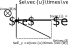
\includegraphics[width=0.9\textwidth]{Hall_forces}
	\caption{Силы, действующие на носитель заряда в проводящей среде в тянущем электрическом и перпендикулярном ему магнитном полях.}
	\label{fig1}
\end{figure}

Если в системе локально течет ток электронов $j_x=nev_{dr\, x}$, направленный вдоль оси $x$, а магнитное поле ${\bf B}$ направлено вдоль оси оси $z$, то на заряды действует действует сила Лоренца ${\bf F_{L}}=e[{\bf v_{dr}B]}$ вдоль оси $y$.
Сила Лоренца должна приводить к образованию компоненты тока вдоль оси $y$, но по условиям ток течет вдоль $x$. Это значит, что заряды должны перераспределиться таким образом, чтобы полностью скомпенсировать силу
Лоренца, создав в $y$ направлении электрическое холловское поле $E_y=v_{dr}B$. Поскольку сила Лоренца
оказывается полностью скомпенсирована $eEy$, то электрон движется так, как если бы магнитного поля не
было, то есть $j_x=E_xbne$, $j_y=j_z=0$. Это позволяет написать в явном виде тензор удельного сопротивления:
\begin{equation}
\widehat{\rho}(B)=\frac{1}{bne}\left(
\begin{tabular}{ccc}
{\it 1} & {\it bB} & {\it 0} \\
{\it -bB} &{\it 1}& {\it 0} \\
{\it 0} &{\it 0}& {\it 1}\\
\end{tabular}
\right).
\label{rhotensor}
\end{equation}

Обращением этой матрицы нетрудно получить тензор проводимости:
\begin{equation}
\widehat{\lambda}(B)=\frac{bne}{1+b^2B^2}\left(
\begin{tabular}{ccc}
{\it 1} & {\it bB} & {\it 0} \\
{\it -bB} &{\it 1}& {\it 0} \\
{\it 0} &{\it 0}& {\it 1}\\
\end{tabular}
\right).
\label{lambdatensor}
\end{equation}

Существуют две основных и принципиально различных геометрии для исследования магнитосопротивления: геометрия
мостика Холла и геометрия диска Корбино (см. Рис \ref{fig2}).

В геометрии мостика Холла ток вынуждают течь вдоль образца, сила Лоренца прибивает носители к краю образца, создавая тем самым холловское поле, которое компенсирует силу Лоренца. Напряжение между точками $V_{xy}$ равно $E_yw$, где, согласно уравнению (\ref{rhotensor}), $E_y=\rho_{yx}\times j_x=j_x B/ne$. Плотность тока, текущего через образец, равна полному току $I$, деленному а площадь поперечного сечения образца $wh$. Таким образом, для холловского напряжения имеем:
\begin{equation}
V_{xy}=\frac{IB}{neh}.
\label{HallVoltage}
\end{equation}

В этой же модели для падения напряжения вдоль образца имеем:
\begin{equation}
V_{xx}=\frac{Il}{nebwh}.
\label{DiagonalVoltage}
\end{equation}

Tаким образом, удельное сопротивление $\rho_{xx}$ образца не зависит от магнитного поля (магнитосопротивление равно 0). Этот факт объясняется тем, что сила Лоренца и сила ЭДС Холла (рис. \ref{fig1}) полностью уравновешивают друг друга. В реальных системах, тем не менее, предположения модели не выполняются и магнитосопротивление зачастую отлично от 0. Причины могут быть различными:
\begin{enumerate}
\item{Система может быть анизотропной. То есть в разных направлениях ($x,y,z$) токопроводящие свойства различны. В этом случае величина силы Лоренца содержит не среднюю дрейфовую скорость, а зависит от направления большой мгновенной скорости электрона.}

\item{Система может быть многокомпонентной. Например, в полупроводниках часто одновременно существуют электроны и дырки, концентрации ($n$ и $p$) и подвижности ($b_n$ и $b_p$) которых в общем случае различаются. Тогда полный тензор проводимости будет суммой тензоров проводимости двух компонент вида \ref{lambdatensor}. Обращением тензора проводимости в пределе малых малых магнитных полей можно показать, что холловское сопротивление двухкомпонентной системы в полупроводнике равно:
      \begin{equation}
      R_{xy}\equiv \frac{V_{xy}}{I}=\frac{n{b_n}^2-p{b_p}^2}{eh(nb_n+pb_p)^2}B
      \label{halltwocomponents}
      \end{equation}
      }

\item{Существуют квантовые эффекты в проводимости, которые приводят к тому, что подвижность зависит от магнитного поля. Например если сам проводящий материал является ферромагнетиком, то с ростом поля он намагничивается, количество доменов уменьшается, а доменные стенки являются причиной сильного рассеяния, то есть уменьшают подвижность. }
\end{enumerate}

Поскольку холловское сопротивление содержит толщину образца $h$, то договорились называть холловское сопротивление, умноженное на толщину образца, постоянной Холла. Постоянная Холла характеризует материал, так как зависит только от концентрации носителей в нем:
$$
R_x=1/ne
$$
 или от соотношений между концентрациями и подвижностями, если в материале несколько типов носителей. В таблице в приложении даны постоянные Холла для различных металлов. Для полупроводников постоянные Холла сильно зависят от наличия малых концентраций примеси и температуры.

Отдельно следует упоямянуть, что существуют двумерные системы (например, графен), в которых движение носителей заряда происходит только в плоскости, а движение в перпендикулярном направлении квантовомеханически запрещено. В этих системах концентрация измеряется в количестве носителей на единицу площади, а холловская постоянная есть просто холловское сопротивление, делённое на магнитное поле. В двумерных системах тензоры в формулах \ref{rhotensor} и \ref{lambdatensor} содержат только $x$ и $y$ компонены, то есть являются матрицами 2х2.

Измерения в геометрии мостика Холла представляют собой четырехконтактные измерения, то есть два контакта используются для задания тока через образец а с двух контактов снимается падение напряжения. Поскольку вольтметр обладает бесконечным сопротивлением (то есть ток через него не течет), измеряемое падение напряжения совершенно не зависит от свойств контактов, а определяется только свойствами материала.

Геометрия диска Корбино представляет собой двухточечную схему. То есть сопротивление образца в ней суммируется с сопротивлениями контактов. Поэтому исключительно важно создать низкоомные контакты к образцу, сопротивлением которых можно пренебречь. В геометрии Корбино из-за аксиальной симметрии не формируется холловское напряжение. Электрическое поле направлено строго по радиусу системы. В магнитном поле ток вынужден протекать под углом к электрическому полю, то есть по спирали. Из-за симметрии полный ток включает только компоненту вдоль радиуса $j_r=\lambda_{xx} E_r$. Плотность тока может быть выражена через полный ток и толщину образца $j_r=Ir_1/(rh)$. Теперь запишем для напряжения:
$$V={\int_{r_1}}^{r_2}E_r dr=1/\lambda_{xx}{\int_{r_1}}^{r_2}j_r dr=Ir_1/(h\lambda_{xx}){\int_{r_1}}^{r_2}1/r dr=Ir_1\ln(r_2/r_1)/(h\lambda_{xx}).$$

Если система однокомпонентная, то магнитосопротивление в геометрии Корбино есть $r_1\ln(r_2/r_1)(1+b^2B^2)/(hneb)$. Для наблюдения этого магнитосопротивления выбирают систему с большой подвижнотью носителей (как правило, это полупроводник с низкой эффективной массой электронов типа InSb)

\begin{figure}
	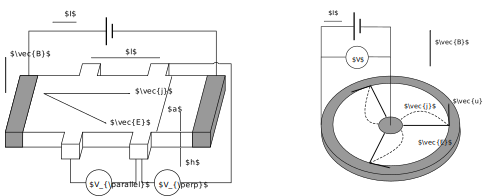
\includegraphics[width=0.9\linewidth]{2schemes}
	\caption{Две геометрии для исследования влияния магнитного поля на проводящие свойства: мостик Холла (слева) и диск Корбино (справа).}
	\label{fig2}
\end{figure}


\end{document}
















При наложении внешнего электрического поля {\bf \it E} электроны начинают ускоряться. Однако после некоторого <<свободного пробега>> происходит соударение с решёткой, электрон теряет набранную энергию, и процесс ускорения начинается заново.
Соударения с решёткой, подобно вязкому трению, приводят к тому, что результирующее движение электрона можно описать
некоторой средней скоростью $\sr{\v{v}}$, пропорциональной внешнему полю:
\begin{equation}
%4
\sr{\vec{v}}=-b\vec{E}.
\end{equation}
Введённая здесь величина $b$ называется \textsf{подвижностью}. В определённых пределах изменения температуры,
напряжённости поля и его частоты эта характеристика вещества остаётся постоянной и приводится в справочниках. Для
положительно заряженных носителей тока в формуле (\r4), очевидно, стоит знак <<плюс>>.

При установившемся движении средняя сила, действующая на электроны со стороны кристаллической решётки, равна внешней силе $-eE$ и направлена в противоположную сторону. Поэтому действие кристаллической решётки на движение электронов в среднем эквивалентно силе трения, пропорциональной скорости:
\begin{equation}
%5
F_{тр}=-\frac{e}{b}\sr{\vec{v}}.
\end{equation}

Если концентрация электронов равна $n$, величина плотности тока определится очевидным соотношением
\begin{equation}
%2
j=en\sr{v}=enbE.
\end{equation}

Таким образом, выполняется закон Ома~--- величина плотности тока $j$ пропорциональна напряжённости поля $E$:
\begin{equation}
%1
j=\sigma E.
\end{equation}

Сравнивая (\r{2}) и (\r{1}), получаем выражение для проводимости
\begin{equation}
%6
\sigma=enb.
\end{equation}

Химически чистые полупроводники обладают проводимостью, которая связана с небольшим числом электронов в зоне
проводимости и таким же числом дырок в валентной зоне. Такая проводимость называется {собственной}~--- она не
связана с~примесями. Добавление небольшого количества специально подобранных примесей (так называемое
{легирование}) может существенно увеличить проводимость полупроводников или даже создать ощутимую проводимость при
комнатной температуре в веществах с запрещённой зоной, ширина которой заметно превышает 2~эВ. Такое происходит, когда атомы примеси имеют энергетические уровни в запрещённой зоне основного материала.

Если заполненные примесные уровни расположены вблизи потолка запрещённой зоны, находящиеся на этих уровнях электронылегко переходят в зону проводимости. Наоборот, на свободные уровни у дна зоны проводимости легко переходят электроны валентной зоны с образованием в этой зоне дополнительного количества дырок. В обоих случаях число переносчиков заряда увеличивается, и проводимость возрастает. В первом случае говорят о полупроводниках {электронного}, или $n$-типа, а во втором~--- о  полупроводниках дырочного, или $p$-типа. В общем случае в процессе электрической проводимости участвуют как электроны, так и дырки. Удельная электрическая проводимость полупроводника при этом равна
\begin{equation}
%7
\sigma=e(nb_e+pb_p),
\end{equation}
где $n$ и $p$~--- концентрации электронов и дырок, а $b_e$ и $b_p$~--- их подвижности. В случае \term{примесной
проводимости} один тип носителей обычно существенно преобладает над другим и в~формуле~(\r7) можно пренебречь одним из слагаемых.


{\small


{\bf \Large Список литераратуры}

\begin{enumerate}
\item{ \emph{Сивухин Д.В.} Общий курс физики.~--- T.~III. Электричество.~--- М.: Наука, 1983. \S\S~86, 95, 98, 100.}
\item{ \emph{Кингсеп А.С., Локшин Г.Р., Ольхов О.А.} Основы физики. Т.~1.~--- М.: Физматлит, 2001. \S\S~8.1--8.3.}
\end{enumerate}

}


{\large \bf 3.3.1 Измерение удельного заряда электрона методами магнитной~фокусировки и~магнетрона}

{\bf Цель работы:}определение отношения заряда электрона к его массе методом магнитной фокусировки и методом магнетрона.



{\LARGE  Метод магнитной фокусировки}

{\bf В работе используются:}{электронно-лучевая трубка и блок питания к ней; соленоид; источник постоянного тока; электростатический вольтметр; милливеберметр; ключи.}

Теоретическая часть работы изложена во введении к разделу в пункте [TO ADD].

Идея опыта заключается в следующем. Электронно-лучевая трубка, вынутая из осциллографа С1-1, помещается в длинный соленоид, создающий магнитное поле, направленное вдоль оси трубки. Электроны вылетают из электронной пушки трубки практически с одинаковыми продольными скоростями $v_{\parallel}$. Небольшое напряжение, подаваемое на отклоняющие пластины, изменяет только поперечную составляющую скорости. Это означает, что все электроны в магнитном поле будут двигаться по спиралям с одним и тем же шагом $L$ и, следовательно, электроны будут встречаться вновь, пересекая ось пучка на расстояниях $L$, $2L$ и т.~д. В~этих точках сечение пучка будет наименьшим, т.~е. в них электронный пучок будет фокусироваться. Следовательно, при изменении магнитного поля изображение пучка на экране будет периодически стягиваться в ярко светящее ся пятнышко. Если расстояние от пушки до экрана $l$, то пучок сфокусируется на экране при условии

$l=nL$, где $n=$1,\, 2,\, 3,\, \ldots,

или
$$
l=\frac{2\pi v_{\parallel}}{(e/m)B_F}n.
$$
Выразив в этой формуле скорость электронов через ускоряющее напряжение, получаем выражение для удельного заряда через измеряемые физические величины:

\begin{equation}
\frac{e}{m}=\frac{8\pi^2V}{l^2}\left(\frac{n^2}{B_F^2}\right).
\label{eq3.1.11}
\end{equation}

{\bf Экспериментальная установка.} Основной частью установки является электронный осциллограф С1-1, трубка которого вынута и установлена в длинном соленоиде, создающим магнитное поле. Напряжение на отклоняющие пластины и питание подводятся к~трубке многожильным кабелем.

\begin{figure}
%\rpic{40mm}
\caption{ Схема измерений по~методу магнитной~фокусировки}
\label{fig3.1.1}
\end{figure}

Пучок электронов, вылетающих из катода с разными скоростями (энергия электрона $\approx 0,1$~эВ), ускоряется анодным напряжением~$\approx 1$~кВ. После прохождения двух диафрагм из пучка выделяются электроны с~практически одинаковой
продольной скоростью $v_{\parallel}$. Небольшое переменное напряжение, поступающее с клеммы <<Контрольный сигнал>>
осциллографа на отклоняющие пластины, изменяет  только поперечную составляющую скорости. Угол~$\alpha$ отклонения пучка от оси трубки, таким образом, зависит  от времени, и электроны прочерчивают на экране трубки светящуюся линию. При увеличении магнитного поля линия на экране сокращается, постепенно стягиваясь в точку, а затем снова удлиняется. Второе прохождение через фокус происходит в том случае, когда электроны на пути от катода к экрану описывают два витка спирали, третье~--- при трёх витках.

Анодное напряжение, определяющее продольную скорость электронов, измеряется электростатическим киловольтметром.

Магнитное поле в соленоиде создаётся постоянным током (\ref{fig3.1.1}), сила которого задается источником питания постоянного тока и измеряется амперметром $A$ источника. Ключ К служит для изменения направления поля в соленоиде.

Величина магнитного поля определяется с помощью измерительной катушки, подключённой к милливеберметру. Этот прибор
измеряет изменение магнитного потока, пронизывающего измерительную катушку, которая намотана  на один каркас с
соленоидом. Описание милливеберметра и правила работы с ним приведены на с.~\pageref{MWB}.

На точность результатов может влиять внешнее магнитное поле, особенно продольное. Оно не вызывает размытия фокуса, но изменяет величину фокусирующего поля. Присутствие внешнего магнитного поля проще всего обнаружить с помощью
переполюсовки соленоида: при изменении направления поля показания милливеберметра будут отличаться, но их полусумма не зависит от наличия постоянного продольного поля.

Измерение магнитного поля с помощью милливеберметра обычно производится в предварительных опытах: при отключении ключа~К устанавливается связь между силой тока, протекавшего через соленоид, и индукцией магнитного поля в соленоиде. По измеренным значениям строится калибровочный график, который используется при обработке результатов основных измерений для пересчёта от тока к индукции магнитного поля.

{\Large \bf ЗАДАНИЕ}

В работе предлагается определить значения магнитных полей, при которых происходит фокусировка электронного пучка, и по результатам измерений рассчитать $e/m$.

\begin{enumerate}
\item{ Ознакомьтесь с назначением ручек управления источника питания по описанию на приборе.}
\item{Познакомьтесь с устройством миливебберметра. См раздел. [ссылка]}
\item{ Прокалибруйте электромагнит~--- определите связь между индукцией~$B$ магнитного поля и током $I$ через обмотки магнита. Для этого с помощью милливеберметра снимите зависимость магнитного потока $\Phi=BSN$, пронизывающего пробную катушку, находящуюся в~магнитном поле, от тока~$I$, измеряемого источником. Значение $SN$ (произведение площади сечения пробной катушки на число витков в ней) указано на установке.

Проведите измерения магнитного потока $\Phi$ во всем диапазоне изменения тока при двух направлениях тока через обмотку.}

\item{ При минимальном или нулевом токе через соленоид включите осциллограф  и подайте напряжение с клеммы <<Контрольный сигнал>> на вертикальный (или горизонтальный) вход усилителя. На экране появится светящаяся линия.}

\item{ Пстепенно увеличивая ток через соленоид, найдите значение тока $I_F$, при котором линия первый раз стягивается в точку (сила тока $I_F$ зависит, конечно, от ускоряющего напряжения $V$, а величина $V$ меняется с изменением яркости луча, поэтому не следует изменять яркость до конца измерений).

     Продолжая увеличивать ток, снимите зависимость $I_F$ от порядкового номера фокуса $n$.}
\item{ Повторите измерения $I_F=f(n)$ для другого направления магнитного поля.}
\item{ Запишите ускоряющее напряжение $V$, величины $L$ и $SN$, указанные на установке, и характеристики приборов. Погрешность миливебберметра зависит от сопротивления измерительной катушки. В нашей установке оно составляет примерно 5 Ом.}
\item{Установите регуляторы источника питания на минимум сигнала и отключите источник. Отключите осциллограф.}
\end{enumerate}

{\rm Обработка результатов}

\begin{enumerate}
\item{Постройте график $B_F=f(I)$.}
\item{По графику $B_F=f(I)$ определите усреднённые значения $B_F$ для каждого фокуса и постройте график зависимости $B_F=f(n)$. Используйте наклон графика для расчёта $e/m$ с помощью формулы~([ссылка]).}
\item{Оцените погрешности и сравните результат с табличным.}

\end{enumerate}


{\Large Измерение ${e/m}$ методом магнетрона}

{\bf В работе используются:}{электронная лампа с цилиндрическим анодом; источники питания лампы и соленоида; соленоид; миллиамперметр; амперметр.}

В настоящей работе отношение $e/m$ для электрона определяется с помощью метода, получившего название <<метод
магнетрона>>. Это название связано с тем, что применяемая в работе конфигурация электрического и магнитного полей
напоминает конфигурацию полей в магнетронах~--- генераторах электромагнитных колебаний сверхвысоких частот.

\begin{figure}
%\noindent\hfil\piccapt{38mm}{3_1_2}
\caption{Схема установки для измерения e/m методом магнетрона}
%\hfil
\label{fig3.1.2}
\end{figure}

\begin{figure}
%\piccapt{45mm}{3_1_3}
\caption{Траектории электронов, вылетающих из~катода, при~разных значениях индукции магнитного~поля}
\label{fig3.1.3}
\end{figure}

Движение электронов в этом случае происходит в кольцевом пространстве, заключённом между катодом и анодом
двухэлектродной электронной лампы (\ref{eq3.1.2}). Нить накала лампы (катод) располагается вдоль оси цилиндрического анода, так что электрическое поле между катодом и анодом имеет радиальное направление. Лампа помещается внутри соленоида, создающего магнитное поле, параллельное оси лампы. Движение электронов в такой лампе рассмотрено в приложении к работе.

Рассмотрим траектории электронов, вылетевших из катода, более подробно. Пусть потенциал анода равен $V_A$. В отсутствие магнитного поля (\ref{eq3.1.1}) электрон движется прямолинейно по радиусу. При слабом поле траектории несколько искривляются, но электроны всё же попадают на анод. При некотором критическом значении индукции магнитного поля $B_{KP}$ траектории искривляются настолько, что только касаются анода. Наконец, при $B>B_{KP}$ электроны вовсе не попадают на анод и возвращаются к катоду. Величину~$B_{KP}$ нетрудно найти по выведенной в приложении формуле (\ref{eq3.1p.18}), заметив, что в этом случае радиальная скорость электрона $\dot{r}$ при $r=r_A$ (при радиусе анода) обращается в нуль:

\begin{equation}
V_A=\frac{eB_{KP}^2r_A^2}{8m}.
\label{eq3.1.19}
\end{equation}

Преобразуя (\ref{eq3.1.19}), найдём

\begin{equation}
\frac{e}{m}=\frac{8V_A}{B_{KP}^2r_A^2}.
\label{eq3.1.20}
\end{equation}

Формула (\ref{eq3.1.20}) позволяет вычислять $e/m$, если при заданном $V_A$ найдено такое значение магнитного поля (или, наоборот, при заданном $B$ такое значение $V_A$), при котором электроны перестают попадать на анод.

\begin{figure}
%\rpic{42mm}{3_1_4}
\caption{Зависимость анодною тока от индукции магнитного поля в соленоиде}
\label{fig3.1.4}
\end{figure}

До сих пор мы рассматривали идеальный случай, когда при $B<B_{кр}$ все электроны без исключения попадают на анод, а при $B>B_{KP}$ все они возвращаются на катод, не достигнув анода. Анодный ток $I_A$ с увеличением магнитного поля изменялся бы при этом так, как это изображено на \ref{fig3.1.4} штриховой линией. В реальных условиях невозможно обеспечить полную коаксиальность анода и катода, вектор индукции магнитного поля всегда несколько наклонён по отношению к катоду, магнитное поле не вполне однородно и т.~д. Все эти причины приводят к сглаживанию кривой на рис. \ref{fig3.1.4} и она приобретает вид сплошной линии. В~хорошо собранной установке перелом функции $I_A=f(B)$ остаётся, однако, достаточно резким и с успехом может быть использован для измерения $e/m$.

{\bf Экспериментальная установка.} Схема установки изображена на рис. \ref{fig3.1.5}. Двухэлектродная лампа Л с цилиндрическим анодом специально изготовлена из немагнитных материалов. Анод лампы состоит из трёх металлических (нержавеющая сталь) цилиндров одинакового диаметра. Два крайних цилиндра электрически изолированы от среднего небольшими зазорами и используются для устранения краевых эффектов на торцах среднего цилиндра, ток с которого используется при измерениях. В качестве катода используется тонкая (диаметром 50~мкм) хорошо натянутая вольфрамовая проволока, расположенная по оси всех трёх цилиндров анодной системы.
Катод лампы разогревается переменным током, отбираемым от стабилизированного источника питания. С этого источника на анод лампы подаётся постоянное напряжение (0--120~В), регулируемое с помощью потенциометра и измеряемое вольтметром $V$.

\begin{figure}
%\fcpic[0.8]{3_1_5}
\caption{Схема измерительной установки}
\label{fig3.1.5}
\end{figure}

Лампа закреплена в соленоиде. Ток, проходящий через соленоид, подаётся с выпрямителя и измеряется амперметром $A$.
Индукция магнитного поля в соленоиде рассчитывается по току, протекающему через обмотку соленоида. Коэффициент
пропорциональности между ними указан на установке.

{\Large \bf ЗАДАНИЕ}

В работе предлагается исследовать зависимость анодного тока от тока, протекающего через соленоид, при различных
напряжениях на аноде лампы и по результатам измерений рассчитать удельный заряд электрона.

\begin{enumerate}
\item{ Установите на аноде лампы потенциал $V_A=60$~В. Снимите зависимость анодного тока $I_A$ от индукции магнитного поля в соленоиде (от тока $I_{M}$ через соленоид). В области резкого изменения тока точки должны лежать чаще (рис. \ref{fig3.1.4})}
\item{ Снимите аналогичные зависимости $I_A=f(I_M)$ для 5--6 фиксированных значений $V_A$ в диапазоне 60--120~В.}

\item{ Запишите параметры установки и характеристики приборов.}
\end{enumerate}

{\rm Обработка результатов}
\begin{enumerate}
\item{Используйте полученные результаты для построения семейства кривых $I_{A}(B)$. Для каждого значения $V_A$ определите по графику критическое значение индукции магнитного поля $B_{KP}$}.
\item Постройте  график зависимости $B_{KR}^2$ от $V_A$. По угловому коэффициенту полученной прямой определите удельный заряд электрона $e/m$. Сравните результат с табличным.
\end{enumerate}

{ \small
{\bf \Large Контрольные вопросы}

\begin{enumerate}
\item{ Нарисуйте и объясните схемы измерения удельного заряда электрона методом магнитной фокусировки и методом магнетрона.}
\item{Объясните принцип действия электронно-лучевой трубки осциллографа.}
\item{ Объясните принцип работы милливеберметра.}
\item{ Почему в методе магнетрона используется анод из трёх цилиндров, а не из одного?}
\end{enumerate}

{\bf \Large Список литераратуры}
\begin{enumerate}
\item{ {\em Сивухин Д.В.} Общий курс физики. Т. III. Электричество.~--- М.: Наука, 1983, \S\S~86, 89.}
\item{ {\em Калашников С.Г.} Электричество.~--- М.: Наука, 1977, \S\S~181--184.}
\end{enumerate}
}



{\LARGE Движение электрона в магнетроне}

Рассмотрим траекторию электронов, движущихся в лампе под действием электрического и магнитного полей. Для вычисленийвоспользуемся цилиндрической системой координат, т.~е. будем характеризовать положение точки расстоянием от оси цилиндра $r$, полярным углом $\phi$ и смещением вдоль оси $z$ (рис.~\ref{fig3.1p.1}). Рассмотрим сначала силы, действующие на электрон со стороны электрического поля. Напряжённость электрического поля в цилиндрическом конденсаторе имеет только радиальную компоненту $E_r=-E$. Поэтому сила, действующая на электрон в таком поле, направлена по радиусу, так что
\begin{equation}
F_r^{el}=eE,\qquad F_z^{el}=F_{\phi}^{el}=0.
\label{eq3.1p.9}
\end{equation}

Рассмотрим теперь силы, действующие на электрон со стороны магнитного поля. Поскольку магнитное поле в нашем случае
направлено по оси $z$, для проекции силы на ось $z$ имеем
\begin{equation}
F_z^{mag}=0.
\label{eq3.1p.10}
\end{equation}

Остальные две составляющие силы найдём с помощью формулы Лоренца. Как нетрудно убедиться,
\begin{equation}
F_{\phi}^{mag}=ev_rB,\qquad F_{r}^{mag}=-ev_{\phi}B.
\label{fig3.1p.11}
\end{equation}

Из простых кинематических соображений ясно, что
\begin{equation}
v_r=\dot{r}=\frac{dr}{dt},\qquad v_{\phi}=r\dot{\phi}=r\frac{d\phi}{dt}.
\label{eq3.1p.12}
\end{equation}

Как видно из формул (\ref{eq3.1p.9}) и (\ref{eq3.1p.10}), ни магнитные, ни электрические силы, действующие на электрон, не имеют составляющих по оси $z$. Движение вдоль оси $z$ является равномерным.

Движение в плоскости ($r$, $\phi$) удобно описывать с помощью уравнения моментов. Для проекции на ось $z$ имеем
\begin{equation}
\frac{dL_{z}}{dt}=M_z,
\label{eq3.1p.13}
\end{equation}

где $L_{z}$~--- момент импульса электрона относительно оси $z$, равный, как известно, $mr^2\dot{\phi}$. Величина $M_z$ равна $rF_{\phi}$. С помощью (\ref{eq3.1p.11}) и (\ref{eq3.1p.13}) найдём
\begin{equation}
M_z=erv_rB.
\label{eq3.1p.14}
\end{equation}

Подставляя (\ref{eq3.1p.12}) и (\ref{eq3.1p.14}) в (\ref{eq3.1p.13}), найдём
\begin{equation}
\frac{d}{dt}\left(mr^2\dot{\phi}\right)=eBr\frac{dr}{dt}=\frac12eB\frac{d(r^2)}{dt}.
\label{eq3.1p.15}
\end{equation}
Интегрируя уравнение (\ref{eq3.1p.15}), получаем

\begin{equation}
r^2\dot{\phi}+A=\frac{eBr^2}{2m},
\label{eq3.1p.16}
\end{equation}

где $A$~--- постоянная интегрирования, которую следует определить из начальных условий. В начале движения радиус $r$ равен радиусу катода, т.~е. очень мал. Правая часть (\ref{eq3.1p.16}) поэтому тоже очень мала. Электроны вылетают из катода с небольшой скоростью, так что $r^{2}\dot{\phi}$ в начальный момент также мало. С хорошей точностью можно поэтому полагать $A=0$. Наше уравнение приобретает при этом простой вид:
\begin{equation}
\dot{\phi}=\frac{eB}{2m}.
\label{eq3.1p.17}
\end{equation}

Рассмотрим теперь движение электрона по радиусу. Работа сил электрического поля, совершаемая при перемещении электрона от катода до точки с потенциалом $V$, равна $W=eV$. Магнитное поле никакой работы не производит. Найденная работа должнабыть поэтому равна кинетической энергии электрона (начальной скоростью электрона мы снова пренебрегаем):
$$
eV=\frac{mv^2}{2}=\frac{(v_r^2+v_\phi^2)}{2m}.
$$
С помощью (\ref{eq3.1p.12}) и (\ref{eq3.1p.17}) найдём
\begin{equation}
eV=\frac{m}{2}\left[\dot{r}^2+\left(\frac{reB}{2m}\right)^2\right].
\label{eq3.1p.18}
\end{equation}
Уравнение (\ref{eq3.1p.18}) полностью определяет радиальное движение электрона.



{\large \bf 3.3.2 Исследование вольт-амперной характеристики вакуумного диода}
{\bf Цель работы:}{определение удельного заряда электрона на основе закона <<трёх вторых>>.}

{\bf В работе используются:}{радиолампа с цилиндрическим анодом; амперметр; многопредельные микроамперметр и вольтметр постоянного тока; стабилизированные источники постоянного тока и постоянного напряжения.}

В работе исследуется зависимость прямого тока, проходящего через вакуумный диод, от напряжения на нём (положительная ветвь вольт-амперной характеристики). Наибольший физический интерес представляет та область положительного напряжения на диоде, в которой пространственный заряд (электронное облако) существенно влияет на распределение электрического поля между катодом и анодом. В этой области ток диода меньше тока эмиссии катода из-за того, что электрическое поле пространственного заряда препятствует движению электронов, испущенных катодом, и часть их возвращается на катод. Как будет показано ниже, в этом случае величина тока пропорциональна напряжению на диоде в степени 3/2:
\begin{equation}
I\propto V^{3/2}
\end{equation}
(<<закон трёх вторых>>). Коэффициент пропорциональности в этой формуле зависит от удельного заряда электрона (отношения заряда электрона к его массе). Цель работы состоит в измерении удельного заряда электрона из вольт-амперной характеристики диода в~области, описываемой <<законом трёх вторых>>.

Рассмотрим прохождение электрического тока через вакуумный диод. Будем считать, что его катод имеет форму нити с
радиусом~$r_K$, а анод~--- форму полого цилиндра с радиусом $r_A$ (рис. \ref{fig3.2.1}). Между катодом и анодом приложена разность потенциалов $V_A$.

\begin{figure}
\caption{Схема расположения электродов в диоде}
\label{fig3.2.1}
\end{figure}

Для простоты примем, что потенциал катода равен нулю, а потенциал анода равен $V_A$. Ток в лампе переносится
электронами, испускаемыми раскалённым катодом. Будем считать, что длина диода намного превосходит его радиальные
размеры, так что электрическое поле можно считать чисто радиальным.

Движение электронов в лампе происходит под действием электрического поля, распределение которого в свою очередь зависит от плотности электронного облака. Нас будет интересовать задача о~стационарном (не меняющемся с течением времени) распределении потенциала и зарядов. Будем также считать, что вследствие симметрии задачи потенциал электрического поля не зависит ни от координаты $z$, ни от угла $\phi$ и является функцией одного радиуса $r$.

Распределение потенциала внутри диода определяется уравнением Пуассона, которое в цилиндрической системе координат имеет вид (как уже сказано, полагаем $\partial V/\partial z=\partial V/\partial\phi=0$):
\begin{equation}
\Delta V=\frac{d^2 V}{dr^2}+\frac{1}{r}\frac{dV}{dr}=-\frac{\rho(r)}{\epsilon_0},
\label{eq3.2.1}
\end{equation}
где $\rho(r)$~--- плотность электрического заряда. Двумя сечениями, перпендикулярными оси $z$, вырежем в диоде слой
толщиной $l$. Плотность заряда $\rho(r)$ связана с током $I$, протекающим через этот слой, очевидной формулой
\begin{equation}
I=-2\pi r\rho(r)v(r)l,
\label{eq3.2.2}
\end{equation}
где $v(r)$~--- скорость электронов на радиусе $r$. В стационарном случае $I$ не зависит от $r$. Таким образом,
\begin{equation}
I=const.
\label{eq3.2.3}
\end{equation}

Скорость электронов определяется разностью потенциалов, которую они прошли, и скоростью их вылета из катода. Этой
последней скоростью мы будем пренебрегать. Ошибка, связанная с указанным предположением, тем меньше, чем выше $V_A$ (при малых напряжениях она может оказаться существенной). Тогда
\begin{equation}
\frac{mv^2(r)}{2}=eV(r).
\label{eq3.2.4}
\end{equation}
В формуле (\ref{eq3.2.4}) $m$~--- масса, $e$~--- абсолютная величина заряда электрона.

Исключая $v$ и $\rho$ из уравнений (\ref{eq3.2.1}), (\ref{eq3.2.2}) и (\ref{eq3.2.4}), найдём
\begin{equation}
r\frac{d^2V}{dr^2}+\frac{dV}{dr}=\frac{I}{2\pi\epsilon_0l}\sqrt{\frac{m}{2eV}}.
\label{eq3.2.5}
\end{equation}

Мы пришли, таким образом, к дифференциальному уравнению второго порядка, из которого следует определить $V$. Это
уравнение может быть решено, если заданы граничные условия, т.~е. значения потенциала на катоде и на аноде.
Дополнительная трудность состоит в том, что неизвестен ток $I$, зависящий от $V$ и входящий в правую часть (\ref{eq3.2.5}), и, таким образом, не полностью определено само уравнение.

Вместо того чтобы задавать величину тока $I$, можно наложить на потенциал ещё одно условие, например, задавать не только потенциал анода, но и производную $dV/dr$ на катоде. Обычно полагают
\begin{equation}
\left.\frac{dV}{dr}\right|_{r=r_K}=0.
\label{eq3.2.6}
\end{equation}
Производная $dV/dr=-E_r$, где $E_r$~--- радиальная компонента напряжённости электрического поля. Наше предположение
означает, таким образом, что вблизи катода пространственный заряд электронов полностью экранирует электрическое поле,создаваемое анодной разностью потенциалов. В электронных лампах при нормальных рабочих режимах электрическое поле обращается в нуль не на самом катоде, а на расстоянии 0,01--0,1~мм от него. В нашем случае этим расстоянием можно пренебречь. Условие (\ref{eq3.2.6}) и пренебрежение начальной скоростью вылетающих с катода электронов не вполне точны и вносятся для упрощения задачи.

Уравнение (\ref{eq3.2.5}) является нелинейным дифференциальным уравнением. Его решение не может быть найдено простыми методами. Пусть, однако, мы нашли решение этого уравнения при некотором $V_A=V_{A0}$ и пусть при этом ток оказался равным $I=I_0$. Покажем, что в этом случае можно найти решение (\ref{eq3.2.5}) и при любом другом значении потенциала $V_A$. Если $I_0$ и $V_{A0}(r)$ являются решением задачи при напряжении $V_{A0}$, то выражения
\begin{equation}
I=I_0\left(\frac{V_A}{V_{a0}}\right)^{3/2},\qquad V(r)=V_{a0}(r)\frac{V_A}{V_{A0}}
\label{eq3.2.8}
\end{equation}
являются искомыми решениями уравнения (\ref{eq3.2.5}) при потенциале~$V_A$. В~самом деле, подставляя (\ref{eq3.2.7}) в (\ref{eq3.2.5}), найдём
$$
r\frac{V_A}{V_{A0}} \frac{d^2V_{A0}(r)}{dr^2}+\frac{V_A}{V_{A0}} \frac{dV_{A0}(r)}{dr}=
\frac{I_0}{2\pi\epsilon_0l} \left( \frac{V_A}{V_{A0}} \right)^{3/2}
\sqrt{ \frac{m}{2eV_{A0}(r )V_A/V_{A0}}}.
$$

Сокращая это уравнение на $V_A/V_{A0}$, придём к уравнению
$$
r\frac{d^2V_{A0}(r)}{dr^2}+ \frac{dV_{A0}(r)}{dr}=\frac{I_0}{2\pi\epsilon_0l}\sqrt{\frac{m}{2eV_{A0}(r)}},
$$
которое, конечно, выполняется, так как по предположению $I_0$ и $V_{A0}(r)$ являются решениями (\ref{eq3.2.5}).

\begin{figure}
\caption{Схема экспериментальной установки}
\label{fig3.2.2}
\end{figure}

Формула (\ref{eq3.2.7}) представляет собой содержание {\em<<закона трёх вторых>>}, утверждающего, что ток в вакуумном диоде пропорционален напряжению на нём в степени 3/2. Этот закон справедлив при любой~--- а не только при цилиндрической~---
геометрии электродов, если ток не слишком велик (т.~е. пока условие (\ref{eq3.2.6}) нарушается не слишком сильно).

В общем случае решение уравнения~(\ref{eq3.2.5}), удовлетворяющее условию (\ref{eq3.2.6}), записывается обычно в виде
\begin{equation}
I=\frac{8\sqrt{2}\pi\epsilon_0l}{9}\sqrt{\frac{e}{m}}\frac{1}{r_A\beta^2}V^{3/2},
\label{eq3.2.8}
\end{equation}

где $\beta^2$~--- функция от $r_A/r_K$, которая может быть задана бесконечным рядом или графиком. То обстоятельство, что$I$ пропорционально $V^{3/2}$, уже обсуждалось. Линейный характер связи между $I$ и $\sqrt{e/m}$ очевиден из
рассмотрения правой части (\ref{eq3.2.5}). Численный коэффициент при $V^{3/2}$ выбран так, чтобы $r_A/r_K\rightarrow\infty$ при$\beta^2\rightarrow 1$.

{\bf Экспериментальная установка.} Исследования проводятся на диоде {2Ц2С} с косвенным накалом. Радиус его катода $r_K=0,9$~мм, радиус анода
$r_A=9,5$~мм, коэффициент $\beta^2=0,98$. Полная высота анода и катода составляет около 20~мм, однако эмиссия электронов происходит только с центральной части катода, покрытой оксидным слоем. Высота этого слоя $l=9$~мм. Поскольку рабочая часть катода достаточно удалена от его торцов, электрическое поле в этой части с~хорошей точностью можно считать радиальным.

Схема экспериментальной установки изображена на Рис. \ref{fig3.2.2}. Для подогрева катода используется стабилизированный выпрямитель {Б5-7}, а в качестве анодного источника~--- выпрямитель Б5-10. В цепь накала включены амперметр $A$ и предохранительное сопротивление $R$. Анодное напряжение измеряется вольтметром (многопредельным гальванометром М-253), а анодный ток~миллиамперметром (микроамперметром М-95 c наружным шунтом). Наружный шунт позволяет изменять пределы измерений тока от 10~мкА до 10~мА.

{\Large \bf ЗАДАНИЕ}

В работе предлагается исследовать вольт-амперные характеристики диода при различных токах накала и по результатам
измерений определить удельный заряд электрона.

\begin{enumerate}

\item{ Ознакомьтесь с экспериментальной установкой, изображённой на рис. \ref{fig3.2.3}.}

\item{ Используя наружный шунт, установите предел измерения миллиамперметра 10~мкА.}

\item{ Установите предел измерения вольтметра 7,5~В.}

\item{ Регулятором выпрямителя цепи накала установите ток накала 1,3~А.}

\item{ Регулятором выпрямителя анодной цепи установите анодное напряжение $V_{A}=0,5$~В.}

\item{ Исследуйте вольт-амперные характеристики диода в диапазоне от 0 до 50~В. В процессе измерений следите за постоянством тока накала. В диапазоне от 0 до 6~В изменяйте напряжение шагами по 0,5~В, в диапазоне от 6 до 10~В~--- шагами по 1~В, а в диапазоне от 10 до 50~В~--- шагами по 5~В.}

\item{ Повторите измерения при токах накала 1,4; 1,5 и 1,6~А.}
\end{enumerate}

{\rm Обработка результатов}
\begin{enumerate}
\item{ По результатам эксперимента постройте графики зависимости $I_A=f(V_{A}^{3/2})$. Определите интервалы значений $V_{A}$, на которых графики имеют вид прямых линий. Найдите  наклон прямолинейных участков характеристик и используйте его для вычисления $e/m$ электрона.}
\item{ В тех же координатах на другом рисунке постройте участок вольт-амперной характеристики в диапазоне анодных напряжений от 0 до 10~В. Почему вольт-амперная характеристика на этом участке нелинейна?}
\end{enumerate}


{\small
{\bf \Large Контрольные вопросы}
\begin{enumerate}

\item{ Нарисуйте качественные графики распределения потенциала $V(r)$ между катодом и анодом: а)~при нулевой разности потенциалов между катодом и анодом; б)~при большой разности потенциалов (режим насыщения тока диода). Объясните эти распределения.}

 \item{Качественно изобразите зависимость тока диода от напряжения на аноде в области от отрицательных напряжений $V_{A}$ до больших положительных. Покажите на этом графике участок напряжений, при которых выполняется <<закон трёх вторых>>. Чем объясняются отклонения от этого закона при малых и больших напряжениях на аноде?}

\item{ Как влияет ток накала катода на ток диода при неизменном напряжении на аноде? Приводит ли это к погрешности
измерения $e/m$?}
\end{enumerate}

{\bf \Large Список литераратуры}

\begin{enumerate}
\item{Сивухин Д.В. Общий курс физики. Т. III. Электричество.~--- М.: Наука, 1983}.
\item{Калашников С.Г. Электричество.М.: Наука, 1977}
\end{enumerate}

{\large \bf 3.3.3 Опыт Милликена.}

{\bf Цель работы:}{измерение элементарного заряда методом масляных капель.}

{\bf В работе используются:}{плоский конденсатор в защитном кожухе, осветитель, измерительный микроскоп, электростатический вольтметр,
электронный секундомер, переключатель напряжения, пульверизатор с маслом.}

{\bf В работе используются:}{плоский конденсатор в защитном кожухе, осветитель, измерительный микроскоп, электростатический вольтметр,
электронный секундомер, переключатель напряжения, пульверизатор с маслом.}

Идея опыта очень проста. Если элементарный заряд действительно существует, то заряд $q$ любого тела может принимать
только дискретную последовательность значений:
\begin{equation}
q=0,\;\pm e,\;\pm 2e,\;\pm 3e,\;\ldots\pm ne,\;\ldots,
\label{eq3.3.1}
\end{equation}

где $e$~--- элементарный заряд. В предлагаемом опыте измеряется заряд небольших капелек масла, несущих всего несколько элементарных зарядов. Сравнивая между собой заряды капель, можно убедиться, что все они по модулю кратны одному и тому же числу, которое равно, очевидно, элементарному заряду.

Для измерения заряда капель будем исследовать их движение в вертикальном электрическом поле.

Движение заряженной капли в электрическом поле зависит как от электрических сил, так и от массы капли. Масса капли можетбыть определена по скорости её падения в отсутствие поля.

Рассмотрим свободное падение капли. Уравнение её движения при падении имеет вид
\begin{equation}
m\frac{dv}{dt}=mg-F_{TP},
\label{eq3.3.2}
\end{equation}

где $m$~--- масса капли, $v$ --- её скорость, $g$~--- ускорение свободного падения, а $F_{TP}$~--- сила вязкого трения капли в воздухе, которая для сферической капли определяется формулой Стокса:
\begin{equation}
F_{TP}=6\pi\eta rv=kv.
\label{eq3.3.3}
\end{equation}

Здесь $r$~--- радиус капли, $\eta$~--- коэффициент вязкости воздуха, $k=6\pi\eta r$. Подставляя (\ref{eq3.3.3}) в (\ref{eq3.3.2}), получим
\begin{equation}
m\frac{dv}{dt}=mg -kv.
\label{eq3.3.4}
\end{equation}
Можно убедиться, что при нулевой начальной скорости решение этого уравнения имеет вид

\begin{equation}
v=\frac{mg }{k}\left(1-e^{-kt/m}\right).
label{eq3.3.5}
\end{equation}
Установившееся значение скорости равно
\begin{equation}
v_{yc}=\frac{mg }{k}=\frac{\frac 43 \pi\rho r^3g }{6\pi\eta r}=\frac29\frac{\rho}{\eta}g r^2,
\label{eq3.3.6}
\end{equation}
где $\rho$~--- плотность масла. Заметим, что (\ref{eq3.3.6}) может быть немедленно получено из (\ref{eq3.3.4}), если положить $dv/dt=0$.

Как следует из (\ref{eq3.3.5}), установление скорости происходит с постоянной времени
\begin{equation}
\tau=\frac{m}{k}=\frac 29 \frac{\rho}{\eta}r^2.
\label{eq3.3.7}
\end{equation}
Время установления скорости, таким образом, быстро падает с уменьшением радиуса капли~$r$. Для мелких капель оно столь мало, что движение капли всегда можно считать равномерным. Выражение (\ref{eq3.3.6}) в этом случае позволяет определить радиус капли, зная скорость её падения. Обозначая через $h$ путь, пройденный каплей за время $t_0$, найдём
\begin{equation}
r=\sqrt{\frac{9\eta h}{2\rho g t_0}}.
\label{eq3.3.8}
\end{equation}

Рассмотрим теперь движение капли при наличии электрического поля плоского конденсатора, пластины которого расположены горизонтально. Напряжённость поля $E$ в конденсаторе равна
\begin{equation}
E=\frac{V}{l},
\label{eq3.3.9}
\end{equation}

где $l$~--- расстояние между пластинами, а $V$~--- разность потенциалов между ними.

Нас будет интересовать случай, когда под действием электрического поля капля поднимается. Уравнение движения при этом примет вид
\begin{equation}
m\frac{dv}{dt}=\frac{qV}{l}-mg -kv,
\label{eq3.3.10}
\end{equation}

где $q$~--- заряд капли. Появление в правой части постоянного слагаемого не изменяет постоянной времени $\tau$. Для
определения установившейся скорости мы можем снова положить левую часть (\ref{eq3.3.10}) равной нулю.

Измерим время $t$ подъёма капли на начальную высоту. Используя равенства (\ref{eq3.3.4}), (\ref{eq3.3.8}) и (\ref{eq3.3.10}), найдём, что заряд капли равен

\begin{equation}
q=9\pi\sqrt{\frac{2\eta^3 h^3}{g \rho}}\cdot\frac{l(t_0+t)}{Vt_0^{3/2} t}.
\label{eq3.3.11}
\end{equation}
Вывод формулы (\ref{eq3.3.11}) предоставляем читателю.

\begin{figure}
%\fcpic[1]{3_3_1}{1}
\caption{Схема экспериментальной установки для измерения заряда электрона}
\label{fig3.3.1}
\end{figure}

{\bf Экспериментальная установка.} Схема установки представлена на рис. \ref{fig3.3.1}. Масло разбрызгивается пульверизатором. Капли масла попадают в~конденсатор~$C$ через небольшое отверстие в верхней пластине. При этом часть из них вследствие трения о воздух приобретает случайный по абсолютной величине и знаку электрический заряд.

Напряжение на пластины подаётся с регулируемого выпрямителя и измеряется вольтметром $V$. Ключ $K$ позволяет менять
направление поля в конденсаторе, чтобы можно было работать  как с отрицательно, так и с положительно заряженными
каплями. При размыкании ключа $K$ конденсатор разряжается через дополнительное сопротивление $R\approx 10$~МОм.

Время отсчитывается по электронному секундомеру.

Естественно, что слабые электрические силы, действующие на каплю, несущую всего
 один или несколько электронных зарядов, способны существенно изменить её движение только в том случае, если сама она очень мала. Опыт производится поэтому с мелкими каплями, наблюдение за которыми возможно только с помощью микроскопа.

В~фокальной плоскости окуляра измерительного микроскопа $M$ виден ряд горизонтальных линий, расстояние между которыми было предварительно определено с помощью объектного микрометра. Наблюдая за перемещением капли между линиями, нетрудно определить путь, пройденный каплей. Время $t_0$ свободного падения капли от одной выбранной линии до другой и время $t$ её обратного подъёма, происходящего под действием сил электрического поля, измеряется электронным секундомером.

Из постановки опыта очевидно, что дискретность заряда может быть обнаружена лишь в том случае, если ошибка $\delta q$ в измерении заряда капли существенно меньше абсолютной величины заряда электрона $e$. Допустимая относительная ошибка опыта $\delta q/q$ должна быть поэтому много меньше $e/q=1/n$, где $n$~--- заряд капли, выраженный в числе зарядов электрона. Этому условию тем легче удовлетворить, чем меньше число~$n$. В нашем случае трудно определить $q$ с точностью лучше 5\%. Заряд капли должен поэтому быть существенно меньше 20~зарядов электрона~--- лучше всего, если он не превосходит пяти электронных зарядов.

Из всех величин, входящих в формулу (\ref{eq3.3.11}), на опыте измеряются только $t_0$, $t$, и $V$. От точности определения этих величин зависит в основном ошибка измерения $q$. Из формулы (\ref{fig3.3.11}) можно найти
\begin{equation}
\frac{\sigma_q}{q}=\sqrt{\frac{\sigma^2_V}{V^2}+\frac{\sigma^2_t t_0^2}{t^2(t_0+t)^2}+
\frac{\sigma^2_{t_0}}{4t^2_0}\left(\frac{3t+t_0} {t+t_0}\right)^2}.
\label{eq3.3.12}
\end{equation}

При $t\approx t_0$ эта формула приобретает вид
\begin{equation}
\frac{\sigma_q}{q}=\sqrt{\frac{\sigma^2_V}{V^2}+ \frac{\sigma^2_t}{4t^2_0}+ \frac{\sigma^2_{t_0}}{t^2_0}}.
\label{eq3.3.13}
\end{equation}

В условиях нашей работы наибольшее влияние на точность эксперимента оказывают два последних стоящих под корнем члена. Ошибка измерения времени $t_0$ и $t$ при визуальном наблюдении капель не может быть сделана меньше 0,1--0,2 секунды. Погрешность в измерении $q$ будет поэтому тем меньше, чем большие значения принимают $t_0$ и $t$. Для увеличения $t_0$ и $t$ можно было бы увеличить расстояние, проходимое каплями, но это сильно усложнило бы экспериментальную установку.
Удобнее идти в другом направлении~--- работать с медленно движущимися каплями, т.е. с каплями малого веса. Время падения $t_0$ таких капель достаточно велико. Чтобы время подъёма $t$ было также достаточно большим, нужно использовать не очень большие разности потенциалов~$V$.

Заметим, что выбор слишком маленьких капель приводит к снижению точности измерений. Броуновское движение малых капель оказывает существенное влияние на их движение и способно заметно исказить картину их падения и подъёма. Маленькие капли могут испаряться, так что их размеры во время наблюдения могут уменьшаться. При малых скоростях движения делаются особенно опасными конвекционные потоки воздуха, которые возникают при неоднородном нагреве установки (происходящем, например, от осветителя камеры). Практически в наших условиях удобно выбирать $t_0\approx t\approx 10$--30~секунд.

Для капель очень малого размера формула Стокса не вполне применима. Использование формулы Стокса без поправок, впрочем, в наших условиях приводит к искажению значений $q$ и $e$ не более чем на 10\% и почти не мешает обнаружению дискретности электрического заряда. Мы рекомендуем поэтому не вводить в формулу никаких поправок.

{\Large \bf ЗАДАНИЕ}

В работе предлагается по измерениям времени свободного падения заряженных капель и времени их подъёма в электрическом поле определить заряд электрона.

\begin{enumerate}

\item{[p3] Перед началом работы оцените с помощью формулы (\ref{eq3.3.11}) величину напряжения~$V$, которое нужно для подъёма капель, несущих от 1 до 5 зарядов электрона на высоту $h=1$~мм, задав $t_0\approx t=20$~с. Если для подъёма капель потребуются меньшие напряжения, то соответствующие капли слишком сильно заряжены и для эксперимента непригодны.

При вычислениях потребуются значения некоторых величин: расстояние между пластинами $l=0,725$~см, плотность масла
$\rho=0,898$~г/см$^3$; коэффициент внутреннего трения воздуха $\eta=1,83\cdot 10^{-4}$~Пуаз~(СГС) или $1,83\cdot 10^{-5}$~Па$\cdot$с
(СИ).}

\item{ Включите осветитель. При этом падающий в камеру свет направлен под углом к оси микроскопа и в объектив не попадает. Поле зрения микроскопа остаётся поэтому тёмным. Капли масла рассеивают свет и кажутся светящимися точками на темном фоне.

Не включая электрическое поле, {\bf слегка} надавите на грушу пульверизатора  и наблюдайте за движением облачка масляных капель в~поле зрения микроскопа (изображение перевёрнуто).}

\item{ Настройте окуляр микроскопа на резкое изображение делений окулярной шкалы. Затем сфокусируйте объектив на появившиеся в рабочем пространстве капли.}

\item{ Наблюдая за движением капель, следует выбирать капли, время падения которых на $h=1$~мм лежит в~пределах
10--30~секунд, и научиться отличать их от более крупных, непригодных для работы. Цена деления окулярной шкалы указана на установке.

В условиях нашей установки регулировкой и коммутацией напряжения занята одна рука наблюдателя. Вторая рука управляет секундомером. Запись результатов измерений ($t_0$, $t$ и $V$) ведёт второй экспериментатор. Наблюдатель быстро устаёт, поэтому рекомендуется периодически меняться местами.

Для уменьшения ошибок в определении $t_0$ и $t$ нужно для пуска и остановки секундомера использовать один и тот же признак~--- всегда нажимать головку секундомера либо в тот момент, когда капля скрывается за линией шкалы, либо, наоборот, когда она появляется из-за линии. Рекомендуется следить за каплей, не отрываясь от окуляра микроскопа, так как в противном случае легко её потерять из виду, и весь эксперимент придётся повторить.}

\item{ В начале опыта следует позволить капелькам свободно падать \mbox{5--10} секунд при выключенном электрическом поле для того, чтобы наиболее крупные капли успели упасть на нижнюю пластину.

Из оставшихся в поле зрения капель выберите одну и произведите с~ней серию измерений, наблюдая её падение под действием силы тяжести и подъём под действием электрического поля. Серия должна состоять из 5--10 измерений $t_0$ и такого же числа измерений $t$ для одной капли.}

\item{ Необходимо проделать не менее 15 таких серий измерений (для 15 различных капель), каждый раз регистрируя величину $V$. При этом нужно иметь в виду, что заряд капли может измениться во время наблюдений; в последнем случае для одной капли получится несколько значений $q$.

Изменение заряда капли может произойти при её подъёме в~электрическом поле. Вычисленное с помощью (\ref{eq3.3.11}) значение заряда будет в этом случае соответствовать некоторому среднему из величины заряда капли в начале и в конце опыта. Соответствующий результат непригоден для обработки и только запутывает опыт. Нужно поэтому стараться вовремя отбросить все случаи, когда перезарядка капли произошла во время её подъёма. Это можно сделать, внимательно наблюдая за движением капли и отбрасывая опыты, в которых капля изменила скорость подъёма во время измерения.}

\item{ Для оценки точности измерений <<подвесьте>> одну из капель в электрическом поле. Определите соответствующее напряжение, отключите его  и измерьте время падения капли на расстояние \mbox{2--3-х} делений шкалы. Поменяв полярность напряжения, верните каплю на прежнее место и снова подвесьте её. Снова запишите напряжение. Повторите  процедуру  для одной капли несколько раз  и на месте  оцените из этого опыта заряд капли по формуле (\ref{eq3.3.11}), полагая время подъёма $t=\infty$. По разбросу результатов ($\Delta V$ и  $\Delta t$) оцените точность измерения заряда этой капли.}

\end{enumerate}


{\rm Обработка результатов}
\begin{enumerate}

\item{ Для всех исследованных капель рассчитайте значения $q$, отложите их на горизонтальной числовой оси и найдите для них общий наибольший делитель. Этот наибольший делитель, вообще говоря, может оказаться равным $e$, $2e$, $3e$ и т.~д.
Однако, чем больше значений $q$ было измерено на опыте, тем меньше вероятность получить в качестве делителя число,
отличное от $e$. Найденное значение $e$ приведите в~системе единиц СИ и в системе СГС.}

\item{ Оцените время релаксации $\tau=v_{yc}/g$ и расстояние $s$, которое прошла бы капля за это время с установившейся скоростью:
$$
s=v_{yc}\tau=\frac{1}{g}\left(\frac{h}{t_0}\right)^2.
$$}

\end{enumerate}

%\newpage

{\small

{\bf \Large Контрольные вопросы}
\begin{enumerate}

\item{ Почему не следует выбирать капли слишком большого и слишком маленького размера?}

\item{ Какие напряжения соответствуют оптимальным условиям опыта? Приведите расчёты.}

\item{ Нарисуйте график зависимости скорости капли в поле силы тяжести от времени и укажите на нём время и путь релаксации.}

\item{ Зная параметры установки, оцените ёмкость конденсатора~$C$ и время его разрядки через сопротивление~$R$ (площадь пластин ${\approx}20$~см$^2$).}

\item{$^*$ Какие ещё способы измерения заряда электрона вам известны?}
\end{enumerate}

{\bf \Large Список литераратуры}

\begin{enumerate}

\item{ {\em Сивухин Д.В.} Общий курс физики. Т.~III. Электричество. --- М.: Наука, 1983. Гл.~V, \S~90.}

\item{ {\em Калашников С.Г.} Электричество.~--- М.: Наука, 1977. Гл.~XVII, \S~178.}
\end{enumerate}
}

{\large \bf 3.3.4 Эффект Холла в полупроводниках}

{\bf Цель работы:}{измерение подвижности и концентрации носителей заряда в полупроводниках.}

{\bf В работе используются:}{электромагнит с источником питания, амперметр, миллиамперметр, милливеберметр, реостат, цифровой вольтметр,
источник питания (1,5~В), образцы легированного германия.}

Элементарная теория свободных носителей заряда в~металлах и полупроводниках изложена во введении к разделу.

{\bf Экспериме
нтальная установка.} Электрическая схема установки для измерения ЭДС~Холла представлена на рис.~\ref{fig3.4.1}.

В~зазоре электромагнита (рис.~\ref{fig3.4.1}а) создаётся постоянное магнитное поле, величину которого можно менять с~помощью регулятора~$R_1$ источника питания электромагнита. Ток питания электромагнита измеряется амперметром~А$_1$. Разъём~К$_1$ позволяет менять направление тока в~обмотках электромагнита.

Градуировка магнита проводится при помощи милливеберметра. Описание милливеберметра и правила работы с ним приведены на с.~\pageref{MWB}.

\begin{figure}
%\fcpic[0.9]{3_4_1}
\caption{Схема установки для исследования эффекта Холла в~полупроводниках}
\label{fig3.4.1}
\end{figure}

Образец из легированного германия, смонтированный в~специальном держателе (рис. \ref{fig3.4.1}б), подключается к~источнику питания ($\simeq 1,5$~В). При замыкании ключа~К$_2$ вдоль длинной стороны образца течёт ток, величина которого регулируется реостатом~$R_2$ и измеряется миллиамперметром~А$_2$.

В образце с током, помещённом в зазор электромагнита, между контактами 3 и 4 возникает разность потенциалов~$U_{34}$, которая измеряется с~помощью цифрового вольтметра.

Иногда контакты 3 и 4 вследствие неточности подпайки не лежат на одной эквипотенциали, и тогда напряжение между ними связано не только с~эффектом Холла, но и с~омическим падением напряжения, вызванным протеканием основного тока  через образец. Измеряемая разность потенциалов при одном направлении магнитного поля равна сумме ЭДС~Холла и омического падения напряжения, а при другом~--- их разности. В~этом случае ЭДС ~Холла~$\epsilon_x$ может быть определена как половина алгебраической разности показаний вольтметра, полученных для двух противоположных направлений магнитного поля в~зазоре. Знак измеряемого напряжения высвечивается на цифровом табло вольтметра.

Можно исключить влияние омического падения напряжения иначе, если при каждом токе через образец измерять напряжение
между точками 3 и 4 в~отсутствие магнитного поля. При фиксированном токе через образец это дополнительное к~ЭДС~Холла напряжение~$U_0$ остаётся неизменным. От него следует (с~учётом знака) отсчитывать величину ЭДС~Холла:
\begin{equation}
\epsilon_x=U_{34}\pm U_0.
\label{fig3.4.1}
\end{equation}
При таком способе измерения нет необходимости проводить повторные измерения с~противоположным направлением магнитного поля.

По знаку $\epsilon_x$ можно определить характер проводимости~--- электронный или дырочный. Для этого необходимо знать
направление тока в~образце и направление магнитного поля.

Измерив ток~$I$ в об
разце и напряжение~$U_{35}$ между контактами~3 и 5 в~отсутствие магнитного поля, можно, зная
параметры образца, рассчитать проводимость материала образца по формуле
\begin{equation}
\sigma=\frac{I\, L_{35}}{U_{35}\,a\,l},
\label{eq3.4.2}
\end{equation}
где $L_{35}$~--- расстояние между контактами 3 и 5, $a$~--- толщина образца, $l$~--- его ширина.

{\Large \bf ЗАДАНИЕ}

В работе предлагается исследовать зависимость ЭДС~Холла от величины магнитного поля при различных токах через образец для определения константы Холла; определить знак носителей заряда и проводимость материала образца.

\begin{enumerate}
\item{ Подготовьте приборы к работе.}

\item{ Проверьте работу цепи питания образца. Ток через образец не должен превышать 1~мА.}

\item{ Проверьте работу цепи магнита. Определите диапазон изменения тока через магнит.}

\item{ Прокалибруйте электромагнит~--- определите связь между индукцией~$B$ магнитного поля в зазоре электромагнита и током $I_M$ через обмотки магнита. Для этого с помощью милливеберметра снимите зависимость магнитного потока $\Phi$, пронизывающего пробную катушку, находящуюся в~зазоре, от тока~$I_M$ ($\Phi=BSN$). Значение $SN$ (произведение площади сечения контура катушки на число витков в ней) указано на держателе катушки.}

\item{ Проведите измерение ЭДС Холла. Для этого вставьте образец в~зазор выключенного электромагнита и определите напряжение~$U_0$ между холловскими контактами 3 и 4 при минимальном токе через образец ($\simeq 0,2$~мА). Это напряжение~$U_0$ вызвано несовершенством контактов~3, 4 и при фиксированном токе через образец остаётся неизменным. Значение~$U_0$ с~учётом знака следует принять за нулевое.

Включите электромагнит и снимите зависимость напряжения~$U_{34}$ от тока~$I_M$ через обмотки магнита при фиксированном токе через образец.

Проведите измерения $U_{34}=f(I_{M})$ при постоянном токе через образец для 6--8 его значений в~интервале 0,2--1~мА. При каждом новом значении тока через образец величина~$U_0$ будет иметь своё значение.

При максимальном токе через образец ($\simeq 1$~мА) проведите измерения $U=f(I_{M})$ при другом направлении магнитного поля.
}
\item{ Определите знак носителей в образце. Для этого необходимо знать направление тока через образец, направление магнитного поля и знак ЭДС Холла.

Направление тока в образце показано знаками~<<+>> и <<$-$>> на рис. \ref{fig3.4.1}. Направление тока в~обмотках электромагнита при установке разъёма~K$_1$ в~положение~I показано стрелкой на торце магнита.

Зарисуйте в тетради образец. Укажите на рисунке направления тока, магнитного поля и отклонение носителей. По знаку
($\pm$) на клеммах цифрового вольтметра определите характер проводимости.
}
\item{Для определение удельной проводимости удалите держатель с~образцом из зазора. Подключите к~клеммам~<<$H_{x}$>> и <<$L_{x}$>> вольтметра потенциальные концы~3 и 5. Измерьте падение напряжения между ними при токе через образец 1~мА.}

\item{ Запишите характеристики приборов и параметры образца $L_{35}$, $a$, $l$, указанные на держателе.}
\end{enumerate}

{\rm Обработка результатов}
\begin{enumerate}

\item {Постройте график зависимости $B=f(I_{M})$.}

\item{ Рассчитайте ЭДС~Холла по формуле~(\ref{eq3.4.1}) и постройте на одном листе семейство характеристик $\epsilon_x=f(B)$ при разных значениях тока~$I$ через образец. Определите угловые коэффициенты~$k(I)=\Delta{\epsilon_x}/\Delta B$ полученных прямых.

Постройте график $k=f(I)$. Рассчитайте угловой коэффициент прямой и по формуле~(TO ADD REF) Приложения определите величину постоянной Холла~$R_{X}$. Рассчитайте концентрацию~$n$ носителей тока в~образце по формуле ([TO ADD REF]).

Оцените погрешность результата и сравните результат с~табличным.}


\item{ Рассчитайте удельную проводимость~$\sigma$ материала образца по формуле~(\ref{eq3.4.2}).

Используя найденные значения концентрации~$n$ и проводимости~$\sigma$, с~помощью формулы~([TO ADD REF]) вычислите подвижность~$b$ носителей тока в~общепринятых для этой величины внесистемных единицах: размерность напряжённости электрического поля $[E]=[U/L]=$~B/см, размерность скорости $[v]=$~см/с, поэтому размерность
подвижности~$[b]=$см$^2$/(В$\cdot$с).

Оцените погрешности и сравните результаты с~табличными.}
\end{enumerate}

{\small

{\bf \Large Контрольные вопросы}
\begin{enumerate}



\item{ Какие вещества называют диэлектриками, проводниками, полупроводниками? Чем объясняется различие их электрических свойств? Как зависит от температуры проводимость металлов и полупроводников?}

\item{ Дайте определение константы Холла. Как зависит константа Холла от температуры у металлов и полупроводников?}

\item{ Зависит ли результат измерения константы Холла от геометрии образца?}

\item{ Как устроен милливеберметр? Зависят ли его показания от сопротивления измерительной катушки? Каким должно быть это сопротивление по сравнению с сопротивлением катушки прибора: большим или маленьким?}

\item{ Получите выражение константы Холла для материалов с~двумя типами носителей. При выводе используйте условие равенства нулю поперечного тока.}

\end{enumerate}

{\bf \Large Список литераратуры}

\begin{enumerate}


\item{ \emph{Сивухин Д.В.} Общий курс физики. Т.~III. Электричество~--- М.: Наука, 1983. \S\S~98, 100.}

\item{ \emph{Парселл Э.} Электричество и магнетизм.~--- М.: Наука, 1983. Гл.~4, \S\S~4--6; Гл.~6, \S~9 (Берклеевский курс физики. Т.~II).
    }

\end{enumerate}
}


{\large \bf 3.3.5 Эффект Холла в металлах}

{\bf Цель работы:}{измерение подвижности и концентрации носителей заряда в металлах.}

{\bf В работе используются:}{электромагнит с источником питания, источник постоянного тока, микровольтметр Ф116/1, амперметры, милливеберметр,
образцы из меди, серебра и цинка.}

Элементарная теория свободных носителей заряда в~металлах и полупроводниках изложена во введении к разделу.

{\bf Экспериментальная установка.} Электрическая схема установки для измерения ЭДС~Холла представлена на рис.~\ref{fig3.5.1}.

\begin{figure}
%\fcpic[0.9]{3_5_1}
\caption{Схема установки для исследования эффекта Холла в~металлах}
\label{fig3.5.1}
\end{figure}

В зазоре электромагнита (рис \ref{fig3.5.1}а) создаётся постоянное магнитное поле, величину которого можно менять с~помощью источника питания электромагнита. Разъём~К$_1$ позволяет менять направление тока в~обмотках электромагнита. Ток питания электромагнита измеряется амперметром~А$_1$.

Градуировка магнита проводится с~помощью милливеберметра. Описание милливеберметра и правила работы с ним приведены на с.~\pageref{MWB}.

Металлические образцы в форме тонких пластинок, смонтированные в~специальных держателях, подключаются к~блоку питания через разъём (рис \ref{fig3.5.1}б). Ток через образец регулируется реостатом~$R_2$ и измеряется амперметром~А$_2$.

Для измерений ЭДС Холла используется микровольтметр Ф116/1, в~котором высокая чувствительность по напряжению сочетается с~малой величиной тока, потребляемого измерительной схемой: минимальный предел измерения напряжения составляет~1,5~мкВ, а потребляемый ток~--- всего~$10^{-8}$~А.

В~образце с~током, помещённом в~зазор электромагнита, между контактами~2 и 4 возникает холловская разность потенциалов, которая измеряется с~помощью микровольтметра, если переключатель К$_3$ подключён к~точке~2 образца. При подключении К$_3$ к~точке~3 микровольтметр измеряет омическое падение напряжения~$U_{34}$, вызванное основным током через образец. При нейтральном положении ключа входная цепь микровольтметра разомкнута.

Ключ К$_2$ позволяет менять полярность напряжения, поступающего на вход микровольтметра.

Иногда контакты~2 и 4 вследствие неточности подпайки не лежат на одной эквипотенциали, и тогда напряжение между ними связано не только с~эффектом Холла, но и с~омическим падением напряжения, вызванным протеканием основного тока через образец. Измеряемая разность потенциалов при одном направлении магнитного поля равна сумме ЭДС~Холла и омического падения напряжения, а при другом~--- их разности. В~этом случае ЭДС Холла $\epsilon_x$ может быть определена как половина
алгебраической разности показаний вольтметра, полученных для двух противоположных направлений магнитного поля в~зазоре.


Можно исключить влияние омического падения напряжения иначе, если при каждом токе через образец измерять
напряжение~$U_0$ между точками~2 и 4 в~отсутствие магнитного поля. При фиксированном токе через образец это
дополнительное к ЭДС Холла напряжение остаётся неизменным. От него следует (с~учётом знака) отсчитывать величину
ЭДС Холла:
\begin{equation}
\epsilon_x=U_{24}\pm U_0.
\label{eq3.5.1}
\end{equation}
При таком способе измерения нет необходимости проводить повторные измерения с~противоположным направлением магнитного поля.

По знаку $\epsilon_x$ можно определить характер проводимости~--- электронный или дырочный. Для этого необходимо знать
направление тока в~образце и направление магнитного поля.

Измерив ток $I$ в образце и напряжение~$U_{34}$ между контактами~3 и 4 в~отсутствие магнитного поля, можно, зная
параметры образца, рассчитать проводимость материала образца по очевидной формуле:

\begin{equation}
\sigma=\frac{I\, L_{34}}{U_{34}\, al},
\end{equation}

где $L_{34}$~--- расстояние между контактами~3 и 4, $a$~--- толщина образца, $l$~--- его ширина.

{\Large \bf ЗАДАНИЕ}

В работе предлагается исследовать зависимость ЭДС~Холла от величины магнитного поля при различных токах через образец для определения константы Холла; определить знак носителей заряда и проводимость различных металлических образцов.

\begin{enumerate}

\item{Подготовьте приборы к работе.}

\item{ Проверьте работу цепи питания образца. Для этого подключите к разъёму блока управления один из образцов~--- медный или серебряный. Убедитесь, что ток через образец можно изменять от 0,5 до 1,2~А.}
\item{ Проверьте работу цепи магнита. Установите разъём К$_1$ в положение I и определите диапазон изменения тока через электромагнит.}
\item{ Прокалибруйте электромагнит. Для этого вставьте в зазор электромагнита пробную катушку милливеберметра и исследуйте зависимость магнитного потока~$\Phi$, пронизывающего пробную катушку, от тока $I_M$ через обмотки магнита ($\Phi=BSN$).
Значение $SN$ (площадь сечения пробной катушки на число витков в ней) указано на держателе катушки.

Проведите измерения магнитного потока для 6--8 значений тока через электромагнит.}

\item{ Проведите измерение ЭДС Холла. Для этого вставьте образец в~зазор выключенного электромагнита и определите напряжение~$U_0$ между холловскими контактами 2 и 4 при минимальном токе через образец ($\simeq 0,5$~А). Это напряжение~$U_0$ вызвано несовершенством контактов~2, 4 и при фиксированном токе через образец остаётся неизменным. Значение~$U_0$ с~учётом знака следует принять за нулевое.

Включите электромагнит и снимите зависимость напряжения~$U_{24}$ от тока~$I_M$ через обмотки магнита при фиксированном токе через образец. Измерения следует проводить при {\bf медленном} увеличении магнитного поля. Резкие изменения магнитного поля наводят ЭДС индукции в~подводящих проводах и вызывают большие отклонения стрелки микровольтметра.

Повторите измерения $U=f(I_{M})$ при постоянном токе через образец для 5--6 его значений в~интервале $0,5-1,2$~А. При каждом новом значении тока через образец величина~$U_0$ будет иметь своё значение.

При максимальном токе через образец проведите измерения $U=f(I_{M})$ при другом направлении магнитного поля.

Для образца из цинка снимите зависимость $U=f(I_{M})$ при одном значении тока через образец ($I\simeq 1$~А).}

\item{Определите знак носителей в образце. Для этого необходимо знать направление тока через образец, направление магнитного поля и знак ЭДС Холла. Направление тока в образце показано знаками~<<+>> и <<$-$>> на рис. \ref{fig3.4.1}. Направление тока в~обмотках электромагнита при установке разъёма~K$_1$ в~положение~I показано стрелкой на торце магнита.

Напомним, что знак потенциала, соответствующий точкам 2 или 4, можно определить по рис. \ref{fig3.4.1}.

Зарисуйте в тетради образец. Укажите на рисунке направление тока, магнитного поля (положение разъёма~K$_1$) и знак
потенциала, соответствующий клемме~4 (положение ключа~K$_2$ при отклонении стрелки вольтметра вправо).

Определите знак носителей заряда для каждого из двух образцов.
}
\item{Определите удельную проводимость образца. Для этого удалите держатель с~образцом из зазора. Установите переключатель микровольтметра <<ПРЕДЕЛЫ ИЗМЕРЕНИЯ>> на 750~мкВ. Ключ~K$_3$ поставьте в~положение~$U_{34}$. При токе через образец~$\sim 1$~А измерьте падение напряжения между контактами 3 и 4 для каждого из двух образцов.}

\item{ Запишите характеристики приборов и параметры образцов $L_{34}$ $a$, $l$, указанные на держателях.}
\end{enumerate}

{\rm Обработка результатов}
\begin{enumerate}
\item{Рассчитайте индукцию магнитного поля~$B$ для каждого значения тока и постройте график зависимости $B=f(I_{M})$.}

\item{Рассчитайте ЭДС Холла по формуле~(\r1) и постройте на одном листе семейство характеристик $\epsilon_x=f(B)$ при разных значениях тока~$I$ через образец (для меди или серебра). Определите угловые коэффициенты~$k(I)=\Delta\epsilon/\Delta B$ полученных прямых.}

\item{ Постройте график $k=f(I)$. Рассчитайте угловой коэффициент прямой и по формуле~([TO ADD REF]) определите величину постоянной Холла $R_x$.

Для цинка изобразите на графике зависимость $\epsilon_x=f(B)$ и по наклону прямой рассчитайте постоянную Холла.

Для обоих образцов рассчитайте концентрацию~$n$ носителей тока по формуле ([TO ADD REF]).

Оцените погрешности и сравните результаты с~табличными.}

\item{ Рассчитайте удельную проводимость~$\sigma$ материала образцов по формуле~(\ref{eq3.5.1}).

Используя найденные значения концентрации~$n$ и проводимости~$\sigma$, с~помощью формулы~([TO ADD REF]) рассчитайте подвижность~$b$ носителей тока в~общепринятых для этой величины внесистемных единицах: размерность напряжённости электрического поля~$[E]=[U/L]=В/см$, размерность скорости~$[v]=см/с$, поэтому размерность подвижности $[b]=$см$^2$/(В$\cdot$с).

Оцените погрешности и сравните результаты с табличными.
}
\end{enumerate}

{\small

{\bf \Large Контрольные вопросы}

\begin{enumerate}

\item{ Какие вещества называют диэлектриками, проводниками, полупроводниками? Чем объясняется различие их электрических свойств? Как зависит от температуры проводимость металлов и полупроводников?}

\item{ Дайте определение константы Холла. Как зависит константа Холла от температуры у~металлов и полупроводников?}

\item{ Зависит ли результат измерения константы Холла от геометрии образца?}

\item{ Как устроен милливеберметр? Зависят ли его показания от сопротивления измерительной катушки? Каким должно быть это сопротивление по сравнению с~сопротивлением рамки прибора: большим или маленьким?}

\end{enumerate}

{\bf \Large Список литераратуры}

\begin{enumerate}


\item{ \emph{Сивухин Д.В.} Общий курс физики. Т.~III. Электричество~--- М.: Наука, 1983. \S\S~98, 100.}

\item{ \emph{Парселл Э.} Электричество и магнетизм.~--- М.: Наука, 1983. Гл.~4, \S\S~4--6; Гл.~6, \S~9 (Берклеевский курс физики. Т.~II).}
\end{enumerate}

}


{\large \bf 3.3.6 Влияние магнитного поля на~проводимость полупроводников}

{\bf Цель работы:}{измерение магнетосопротивления полупроводниковых образцов различной формы.}

{\bf В работе используются:}{электромагнит, милливеберметр, цифровой вольтметр, амперметр, миллиамперметр, реостат, образцы монокристаллического антимонида индия (InSb) $n$-типа.}

Элементарная теория свободных носителей заряда в металлах и полупроводниках изложена во введении.

\begin{figure}
%\fcpic[0.9]{3_6_1}
\caption{Схема установки для~исследования влияния магнитного~поля на~проводимость полупроводников}
\label{fig3.6.1}
\end{figure}

{\bf Экспериментальная установка.} Схема установки для исследования магнетосопротивления полупроводников и геометрического резистивного эффекта представлена на рис. \ref{fig3.6.1}.

В~зазоре электромагнита (рис. \ref{fig3.6.1}а) создаётся постоянное магнитное поле. Ток питания магнита подаётся от сети (${=}120$~В), регулируется реостатом~$R_1$ и измеряется амперметром~$A_1$.

Магнитная индукция в зазоре измеряется при помощи милливеберметра. Описание милливеберметра и правила работы с ним приведены на с.~\pageref{MWB}.

Образец в форме кольца (диск Корбино) или пластинки, смонтированный в~специальном держателе, подключается к~источнику постоянного напряжения 5~В. При замыкании ключа~К$_2$ сквозь образец течёт ток, величина которого измеряется миллиамперметром $A_2$ и регулируется реостатом $R_2$. Балластное сопротивление $R_0$ ограничивает ток через образец. Измеряемое напряжение подаётся на вход цифрового вольтметра.

{\Large \bf ЗАДАНИЕ}

В работе предлагается при постоянном токе через образец исследовать зависимость напряжения на образце от величины магнитного поля и от ориентации образца в магнитном поле; по результатам измерений рассчитать подвижность электронов, удельное сопротивление материала образца и концентрацию электронов.

\begin{enumerate}

\item{ Подготовьте приборы к работе.}

\item{ Концы от точек 3 и 4 разъёма подсоедините к клеммам вольтметра.}

\item{ Присоедините диск Корбино через разъём к цепи питания. Определите диапазон изменения силы тока через образец.}

\item{ Определите диапазон изменения силы тока через электромагнит и подберите подходящий предел измерений амперметра~$A_1$.}

\item{ Прокалибруйте электромагнит~--- с помощью милливеберметра исследуйте зависимость индукции~$B$ магнитного поля в зазоре от тока $I_M$ через обмотки магнита. Для расчёта индукции измерьте поток~$\Phi$ вектора магнитной индукции, который пронизывает пробную катушку, находящуюся в~зазоре ($\Phi=BSN$). Значение $SN$ (площадь сечения контура катушки на число витков в ней) указано на держателе катушки.}

\item{ Проведите измерения магнитного потока для 6--8 значений тока $I_M$ через электромагнит.}

\item{ Исследуйте магнетосопротивление образцов. Для этого вставьте диск в~зазор выключенного электромагнита и установите ток через образец~$I_0=25$~мА. Измерьте падение напряжения $U_0$ на образце.}

\item{ Включите электромагнит и снимите зависимость напряжения~$U$ на образце от тока~$I_M$ через обмотки магнита при фиксированном токе~$I_0=25$~мА через образец.}

\item{ Проверьте, что результат измерения не зависит от направления магнитного поля.}

\item{ Вместо диска Корбино подключите к~измерительной цепи образец, имеющий форму пластинки. Поместите образец в зазор выключенного электромагнита и измерьте падение напряжения $U_0$ на образце при токе через образец~$10$~мА.}

\item{ Включите электромагнит и снимите зависимость напряжения~$U$ на образце от тока через магнит при постоянном токе~$I=10$~мА. При измерениях длинная сторона образца должна быть направлена поперёк поля, а средняя (ширина) в~одной серии опытов располагается вдоль, а в другой~--- поперёк поля.}

\item{ Запишите размеры диска и характеристики приборов.}
\end{enumerate}

{\rm Обработка результатов}
\begin{enumerate}





\item { Рассчитайте индукцию магнитного поля и постройте график зависимости~$B=f(I_{M})$.}

\item { На одном листе постройте графики для всех трёх серий, отложив по оси~$X$ величину~$B^2$, а по оси~$Y$~--- $(U-U_0)/U_0$.}

\item { По наклону прямолинейного участка графика для диска Корбино рассчитайте с~помощью формул ([TO ADD REF] ) и ([TO ADD REF]) подвижность носителей.}

\item { Вычислив сопротивление диска в отсутствие магнитного поля и зная геометрические размеры образца, рассчитайте удельное сопротивление материала образца $\rho_0$ по формуле ([TO ADD REF]).

С помощью формулы ([TO ADD REF]) найдите концентрацию носителей тока.}

\item { Оцените погрешности и сравните результаты с табличными.}
\end{enumerate}

{

\small

{\bf \Large Контрольные вопросы}
\begin{enumerate}


\item{ Исследуйте уравнения движения электронов в прямоугольной пластинке. Зависит ли сопротивление пластинки от индукции магнитного поля?}

\item{ Поясните качественно (без формул), почему сопротивление образца зависит от магнитного поля.}
\end{enumerate}

{\bf \Large Список литераратуры}

\begin{enumerate}

\item{ \emph{Сивухин Д.В.} Общий курс физики. Т.~III. Электричество~--- М.: Наука, 1983. \S\S~98, 100.}

\item{ \emph{Парселл Э.} Электричество и магнетизм.~--- М.: Наука, 1983. Гл.~4, \S\S~4--6; Гл.~6, \S~9 (Берклеевский курс физики. Т.~II).}

\end{enumerate}
}

\bigskip

\noindent\hfil{\large\bf  МИЛЛИВЕБЕРМЕТР}\label{MWB}

{\large\bf  Устройство и принцип действия}

Милливеберметр (флюксметр) служит для измерения постоянного во времени магнитного потока. Это прибор
магнитоэлектрической системы, работающий в баллистическом режиме: рамка с током вращается в поле постоянного магнита; отклонение рамки пропорционально заряду, если через неё пропускается короткий импульс тока. От обычных гальванометров постоянного тока милливеберметр отличается тем, что на его рамку не действуют никакие упругие силы, поэтому его подвижная часть находится в~безразличном равновесии.

\begin{figure}
%\rpic{3.0cm}{mwb-01}
\caption{Рамка в~магнитном поле}
\label{fig3.MWB.1}
\end{figure}

В цепь рамки прибора включается наружная измерительная (пробная) катушка. При изменении магнитного потока,
пронизывающего эту катушку, в ней возникает ЭДС индукции, и по цепи рамки течёт индукционный ток. При этом отклонение рамки, независимо от её начального положения, пропорционально изменению магнитного потока $\Delta\Phi$ и может служить для его измерения.

Рассмотрим работу милливеберметра. Уравнение вращательного движения рамки имеет вид
\begin{equation}
J\ddot{\phi}=M,
\label{fig3.MWB.1}
\end{equation}

где $J$~--- момент инерции рамки милливеберметра, $\phi$~--- угол её поворота (рис. \ref{fig3.MWB.1}). Момент сил $M$ определяется путём умножения силы $F=IlNB_0$, действующей на каждую из продольных сторон рамки (направленных вдоль оси вращения), на удвоенное плечо, т.е. на поперечный размер рамки $a$, здесь $I$~--- сила тока в рамке, $l$~--- длина продольной стороны,$N$~--- число витков намотанного на рамку провода, $B_0$~--- индукция поля постоянного магнита милливеберметра. Поле магнита радиально, это обеспечивает равномерность шкалы прибора. Таким образом,
$$
J\ddot{\varphi}=ISNB_0,
$$
где $S=la$~--- площадь рамки. Введя обозначение $K=SNB_0$, получим

\begin{equation}
J\ddot{\varphi}=KI.
\label{fig3.MWB.2}
\end{equation}

Вычислим теперь ток $I$. Этот ток генерируется под действием как внешней ЭДС индукции $\epsilon_K$, возникающей в измерительной катушке, так и внутренней $\epsilon_P$, возникающей в рамке при её движении в магнитном поле:
\begin{equation}
RI=\epsilon_K+\epsilon_P,
\label{fig3.MWB.3}
\end{equation}

где $R$~--- полное сопротивление цепи рамки.

Внешняя ЭДС $\epsilon_K$ наводится в измерительной катушке при изменении проходящего сквозь неё магнитного потока~$\Phi$:
\begin{equation}
\epsilon_K=-\frac{d\Phi}{dt},
\label{eq3.MWB.4}
\end{equation}

а $\epsilon_P$ возникает в продольных сторонах рамки при их движении в поле постоянного магнита со скоростью $v=\dot{\phi}a/2$:

\begin{equation}
\epsilon_P=-SNB_0\dot\phi=-K\dot\phi.
\label{eq3.MWB.5}
\end{equation}

Подставим (\ref{eq3.MWB.3})~--~(\ref{eq3.MWB.5}) в (\ref{eq3.MWB.2}), и уравнение движения рамки принимает вид

\begin{equation}
\frac{JR}{K^2}\ddot{\phi}+\dot{\phi}=-\frac{1}{K}\dot{\Phi}.
\label{eq3.MWB.6}
\end{equation}

Проинтегрируем это уравнение по времени:
\begin{equation}
\frac{JR}{K^2}(\dot{\phi_2}-\dot{\phi_1})+(\phi_2-\phi_1)=-\frac{1}{K}(\Phi_2-\Phi_1).
\label{eq3.MWB.7}
\end{equation}
Для измерения магнитного потока с помощью милливеберметра можно:

а) вынести измерительную катушку из области измеряемого в область нулевого поля;

б) оставив катушку в поле неподвижной, отключить измеряемое поле.

В любом  из этих вариантов скорость изменения потока $\dot{\Phi}$ в начале и в конце опыта равна нулю. В начале опытарамка милливеберметра не движется, так что $\dot{\phi}_1=0$. Покажем, что и $\dot{\phi}_2=0$.

В~самом деле, при $\dot{\Phi}=0$ в уравнении (\ref{eq3.MWB.6}) пропадает правая часть. В отсутствие внешних сил рамка рано или поздно должна остановиться вследствие действия сил электромагнитного торможения. Можно найти закон движения при торможении, решив дифференциальное уравнение (\ref{eq3.MWB.6}):
\begin{equation}
\dot{\phi}=\dot{\phi}(0)\,\exp\left(-\frac{K^2}{JR}t\right),
\label{eq3.MWB.8}
\end{equation}
где $\dot{\phi}(0)$~--- начальная угловая скорость рамки. При больших $t$ угловая скорость $\dot{\phi}$ оказывается экспоненциально мала, т.~е. $\dot{\phi}_2\rightarrow 0$.

Подставляя $\dot{\phi}_1=0$ и $\dot{\phi}_2=0$ в (\ref{eq3.MWB.7}), найдём
\begin{equation}
\phi_2-\phi_1=-\frac{1}{K}(\Phi_2-\Phi_1).
\label{eq3.MWB.9}
\end{equation}

Таким образом, \emph{угол отклонения рамки милливеберметра пропорционален изменению магнитного потока, пронизывающего измерительную катушку}. Коэффициент пропорциональности выбирается так, что шкала прибора градуируется в милливеберах.Разделив поток на площадь и число витков измерительной (пробной) катушки, мы определим индукцию $B$ внешнего магнитного поля.

\begin{figure}
%\rpic{4.5cm}{mwb-02}
\caption{Схема прибора}
\label{fig3.MWB.2}
\end{figure}

Обратим внимание на структуру формулы (\ref{eq3.MWB.8}). Время $t$, в течение которого затухает движение рамки, должно быть небольшим, т.к. рамка находится в~безразличном равновесии и склонна дрейфовать. Самопроизвольное перемещение стрелки искажает результаты измерений. Из (\ref{eq3.MWB.8}) видно, что время успокоения прибора падает с уменьшением $R$, поэтому
\emph{милливеберметр работает правильно лишь при замыкании его рамки на достаточно малое сопротивление}. Допустимая величина сопротивления измерительной катушки указана на приборе.

Принципиальная схема милливеберметра изображена на рис \ref{fig3.MWB.2}. Так как прибор не имеет противодействующего механического момента, стрелка его после измерения не возвращается к начальному положению. Для установки стрелки на нужную отметку служит электромагнитный \emph {корректор}~--- вторая магнитная система, состоящая из постоянного магнита и сердечника с обмоткой. Когда ручка переключателя находится в положении <<Корректор>>, обмотка корректора замкнута на рамку прибора, в которой в момент поворота ручки корректора (вследствие пересечения силовых линий магнита корректора) возникает ток.
Изменяя направление и угол поворота ручки корректора, можно установить стрелку прибора на любом делении шкалы.

При положении ручки переключателя на отметке <<Арретир>> рамка прибора замкнута накоротко, и подвижная система прибора находится в сильно успокоенном режиме.

В положении <<Измерение>> прибор готов к работе.

%\newpage

{\large \bf Правила работы}

\vskip-\lastskip

{\textsf{Общие указания}}

\begin{enumerate}

\item{Для измерения магнитного потока подключённая к прибору измерительная катушка помещается в магнитное поле перпендикулярно ему.}

\item{Для исключения погрешности от паралакса отсчёт показаний следует проводить так, чтобы изображение стрелки в зеркале шкалы совпадало с самой стрелкой.}
\end{enumerate}

{\textsf{Измерение магнитного потока}}

\begin{enumerate}

\item{Поставьте переключатель в положение <<Корректор>> и поворотом рукоятки корректора установите начальное положение стрелки, удобное для измерений.

Если ручка корректора дошла до упора, а стрелка сместилась недостаточно, поверните рукоятку корректора в обратную сторону до упора, а затем снова поворачивайте её, пока стрелка не встанет на нужное деление.}

\item{Поставьте переключатель в положение <<Измерение>>. Заметьте начальное положение стрелки (вся шкала --- 10 дел. --- 10~mWb).

Измените магнитный поток сквозь катушку до нуля и заметьте новое положение стрелки. Разность показаний определяетмагнитный поток.

Изменять магнитный поток рекомендуется одним из способов:

а) быстро удаляя пробную катушку из области действия магнитного поля на расстояние, где магнитный поток практически равен нулю (рекомендуется);

б) выключая магнитное поле, если катушка закреплена жёстко.

Не рекомендуется переполюсовывать магнит для измерений поля, т.~к. при этом часто ломаются переключатели.

Величина $SN$, необходимая для расчёта индукции поля, указана на пробной катушке.}

\item{По окончании работы следует заарретировать прибор~--- поставить переключатель в положение <<Арретир>>.}

\item{Не реже одного раза в месяц рекомендуется проверять состояние приборов по образцовому прибору.}

%Один раз в два года, а также после каждого ремонта, приборы должны проверяться в местном отделении Комитета %стандартов, мер и измерительных приборов.

\end{enumerate}
